\documentclass[12pt,a4paper]{report}
\usepackage[top=2.5cm, bottom=2.5cm, left=2.5cm, right=2.5cm]{geometry}

% Diff?rentes options pour la classe :
% - taille de la fonte    : 10pt, 11pt, 12pt
% - recto ou recto-verso    : oneside, twoside
% - stade de d?veloppement    : draft, final


\usepackage[english]{babel}
%\usepackage[latin1]{inputenc}    % Pour utiliser les lettres accentu?es
\usepackage{bookmark}
%\usepackage[utf8]{inputenc}%           gestion des accents (source)
%\usepackage[T1]{fontenc}%              gestion des accents (PDF)
%\usepackage[francais,english]{babel}%          gestion du fran?ais
\usepackage{textcomp}%                 caract?res additionnels
\usepackage{indentfirst}
\usepackage[pdftex]{graphicx}
\usepackage{setspace}
\usepackage{hyperref}
\usepackage[french]{varioref}
\usepackage{fancyhdr}
\usepackage{color}
\usepackage{colortbl}
\usepackage{amsmath}
\usepackage{ifpdf} % part of the hyperref bundle
\usepackage{array}
\usepackage{longtable}
\usepackage{float}
\usepackage{amsmath}
\usepackage{booktabs}
\usepackage{makecell}


\setlength{\headheight}{15pt} % slightly larger than the minimum required
%\usepackage{abstract}


 % set fonts for nicer pdf view
 \IfFileExists{lmodern.sty}{\usepackage{lmodern}}{}
 
\pagestyle{fancy}
\fancyhead[L]{\nouppercase\leftmark} %pour afficher le nom du chapitre ? gauche
\fancyhead[C]{}
\fancyhead[R]{\nouppercase\rightmark} %pour afficher le nom de la section ? droite


\fancyfoot[L]{}
\fancyfoot[C]{}
\fancyfoot[R]{\textbf{\thepage}}

% D?but du document
\begin{document}

%%%%%%%%%%%%%%%%%%%%%%%%%%%%%%%%%%%%%%%%%
% University Assignment Title Page 
% LaTeX Template
% Version 1.0 (27/12/12)
%
% This template has been downloaded from:
% http://www.LaTeXTemplates.com
%
% Original author:
% WikiBooks (http://en.wikibooks.org/wiki/LaTeX/Title_Creation)
%
% License:
% CC BY-NC-SA 3.0 (http://creativecommons.org/licenses/by-nc-sa/3.0/)
% 
% Instructions for using this template:
% This title page is capable of being compiled as is. This is not useful for 
% including it in another document. To do this, you have two options: 
%
% 1) Copy/paste everything between \begin{document} and \end{document} 
% starting at \begin{titlepage} and paste this into another LaTeX file where you 
% want your title page.
% OR
% 2) Remove everything outside the \begin{titlepage} and \end{titlepage} and 
% move this file to the same directory as the LaTeX file you wish to add it to. 
% Then add \input{./title_page_1.tex} to your LaTeX file where you want your
% title page.
%
%%%%%%%%%%%%%%%%%%%%%%%%%%%%%%%%%%%%%%%%%



\begin{titlepage}

\newcommand{\HRule}{\rule{\linewidth}{0.5mm}} % Defines a new command for the horizontal lines, change thickness here

\center % Center everything on the page
 
%----------------------------------------------------------------------------------------
%	HEADING SECTIONS
%----------------------------------------------------------------------------------------


\begin{minipage}[l]{0.2\columnwidth}

\includegraphics[width=3cm,height=2cm]{assets/logo_istic.jpg}\\
\end{minipage}
\hfill
\begin{minipage}[l]{0.5\columnwidth}
\centering
\footnotesize
\textbf{\textsc{Republic of Tunisia}}\\
\textbf{\textsc{The Ministry of Higher Education \\
and Scientific Research}}\\
\medskip 
\textbf{\textsc{The University of Carthage}}\\
\medskip 
\textbf{\textsc{The Higher Institute of Information and Communication Technologies}}
\end{minipage}
\hfill
\begin{minipage}[l]{0.2\columnwidth}

\includegraphics[width=3cm,height=2cm]{assets/logo_ucar.jpg}\\
\end{minipage}

\vskip1cm
\textsc{\large END-OF-STUDY PROJECT REPORT}\\[0.5cm] % Minor heading such as course title\\

\textbf{Submitted in Partial Fulfillment of the  Requirements for the }

\textsc{\large Bachelor Degree in Computer Science
}\\[0.5cm] % Minor heading such as course title\\

\textbf{Field of Study : Software Engineering and Information Systems}

\vskip1cm%

%----------------------------------------------------------------------------------------
%	TITLE SECTION
%----------------------------------------------------------------------------------------

\HRule \\[0.4cm]
\textcolor{blue}{\large \bfseries Design and Development of an AI-Powered Feasibility Analysis Suite with Integrated Chatbot Assistance for Public-Private Partnership (PPP) Evaluations}\\[0.2cm] % Title of your document
\HRule \\[1cm]

\vskip0.5cm%
\textit{By}\\
\textsc{\large Yassine HACHANI AND Ahmed HAJJEM}\\[0.5cm] % Minor heading
\vskip0.5cm%

%\vspace{0.5cm}
%\begin{center}
{Conducted within....}\\
%\smallskip

\includegraphics[width=0.2\columnwidth]{assets/jade_advisory.jpg}\\
%\end{center}

\vskip1cm
 
%----------------------------------------------------------------------------------------
%	Supervisor SECTION
%----------------------------------------------------------------------------------------
 \begin{flushleft}
Publicly defended on May 25, 2024 in front of the jury members:
\smallskip

\begin{minipage}[c]{0.3\columnwidth}
Chairman:\\
Reporter:\\
Examiner:\\
Professional Supervisor:\\
Academic Supervisor:
\end{minipage}
%\hfill
\begin{minipage}[c]{0.6\columnwidth}
Name SURNAME, University Relations Leader, IBM\\
Name SURNAME, Teacher, ISTIC\\
Name SURNAME, Teacher, ISTIC\\
Name SURNAME, Engineer, VERMEG\\
Name SURNAME, Teacher, ISTIC
\end{minipage}
%\begin{minipage}[c]{0.4\columnwidth}
%{\small Maitre-Assistant en Informatique}\\
%{\small Maitre-Assistant en Informatique}\\
%{\small Maitre-Assistant en T�l�communications}\\
%{\small Ing�nieur}\\
%{\small Assistant en Informatique}
%\end{minipage}
 \end{flushleft}

%----------------------------------------------------------------------------------------
%	DATE SECTION
%----------------------------------------------------------------------------------------
\vskip1.5cm

{\large Academic Year: 2023-2024}\\[3cm] 


\vfill % Fill the rest of the page with whitespace

\end{titlepage}
%\end{document}
%%%%%%%%%%%%%%%%%%%%%%%%%%%%%%%%%%%%%%%%%
% University Assignment Title Page 
% LaTeX Template
% Version 1.0 (27/12/12)
%
% This template has been downloaded from:
% http://www.LaTeXTemplates.com
%
% Original author:
% WikiBooks (http://en.wikibooks.org/wiki/LaTeX/Title_Creation)
%
% License:
% CC BY-NC-SA 3.0 (http://creativecommons.org/licenses/by-nc-sa/3.0/)
% 
% Instructions for using this template:
% This title page is capable of being compiled as is. This is not useful for 
% including it in another document. To do this, you have two options: 
%
% 1) Copy/paste everything between \begin{document} and \end{document} 
% starting at \begin{titlepage} and paste this into another LaTeX file where you 
% want your title page.
% OR
% 2) Remove everything outside the \begin{titlepage} and \end{titlepage} and 
% move this file to the same directory as the LaTeX file you wish to add it to. 
% Then add \input{./title_page_1.tex} to your LaTeX file where you want your
% title page.
%
%%%%%%%%%%%%%%%%%%%%%%%%%%%%%%%%%%%%%%%%%



\begin{titlepage}

\newcommand{\HRule}{\rule{\linewidth}{0.5mm}} % Defines a new command for the horizontal lines, change thickness here

\center % Center everything on the page
 
%----------------------------------------------------------------------------------------
%	HEADING SECTIONS
%----------------------------------------------------------------------------------------


\begin{minipage}[l]{0.2\columnwidth}

\includegraphics[width=3cm,height=2cm]{assets/logo_istic.jpg}\\
\end{minipage}
\hfill
\begin{minipage}[l]{0.5\columnwidth}
\centering
\footnotesize
\textbf{\textsc{Republic of Tunisia}}\\
\textbf{\textsc{The Ministry of Higher Education \\
and Scientific Research}}\\
\medskip 
\textbf{\textsc{The University of Carthage}}\\
\medskip 
\textbf{\textsc{The Higher Institute of Information and Communication Technologies}}
\end{minipage}
\hfill
\begin{minipage}[l]{0.2\columnwidth}

\includegraphics[width=3cm,height=2cm]{assets/logo_ucar.jpg}\\
\end{minipage}

\vskip1cm
\textsc{\large END-OF-STUDY PROJECT REPORT}\\[0.5cm] % Minor heading such as course title\\

\textbf{Submitted in Partial Fulfillment of the  Requirements for the  }

\textsc{\large Bachelor Degree in Computer Science
}\\[0.5cm] % Minor heading such as course title\\

\textbf{Field of Study : Software Engineering and Information Systems}

\vskip1cm%

%----------------------------------------------------------------------------------------
%	TITLE SECTION
%----------------------------------------------------------------------------------------

\HRule \\[0.4cm]
\textcolor{blue}{ \large \bfseries Design and Development of an AI-Powered Feasibility Analysis Suite with Integrated Chatbot Assistance for Public-Private Partnership (PPP) Evaluations}\\[0.2cm] % Title of your document
\HRule \\[1cm]

\vskip0.5cm%
\textit{By}\\
\textsc{\large Yassine HACHANI AND Ahmed HAJJEM}\\[0.5cm] % Minor heading
\vskip0.5cm%

%\vspace{0.5cm}
%\begin{center}
{Conducted within....}\\
%\smallskip

\includegraphics[width=0.2\columnwidth]{assets/jade_advisory.jpg}\\
%\end{center}
\vskip1cm
 
%----------------------------------------------------------------------------------------
%	Supervisor SECTION
%----------------------------------------------------------------------------------------


 \begin{flushleft}
\textbf{\textsc{Authorization of  graduation project report submission:}}\\[0.5cm] % Minor heading
\vskip0.5cm
\begin{minipage}[c]{0.3\columnwidth}
Professional Supervisor:\\
\vskip0.5cm
Issued on :\\
\vskip0.5cm
Signature:\\

\end{minipage}
\hfill
\begin{minipage}[c]{0.4\columnwidth}
Academic Supervisor:\\
\vskip0.5cm
Issued on :\\
\vskip0.5cm
Signature:\\
\end{minipage}

 \end{flushleft}

%----------------------------------------------------------------------------------------
%	DATE SECTION
%----------------------------------------------------------------------------------------
%\vskip1cm
%{\large Ann�e Universitaire: 2021-2022}\\[3cm] 



\vfill % Fill the rest of the page with whitespace

\end{titlepage}
%\end{document}
\newpage
\pagenumbering{roman}
\chapter*{Dedicace}
\addcontentsline{toc}{chapter}{Dedicace}

\noindent A mes parents,
\\
A ma famille,
\\
A mes amis 

\chapter*{Dedicace}
\addcontentsline{toc}{chapter}{Dedicace}

A mes parents,
A mes frères et s\oe urs,
A mes amis 


\chapter*{Remerciements}
\addcontentsline{toc}{chapter}{Remerciements}

Je tiens à remercier 


\chapter*{Key Terms}
\addcontentsline{toc}{chapter}{Key Terms}
%give me a solution for this tex file to remove the space shown between the text at \textbf and the ':' 

\begin{itemize}
 \item Attention: Statistical apparatus for evaluating the impact of each token fed through an LLM.
\item \textbf{Cohere:} is a Canadian multinational technology company focused on enterprise artificial intelligence, specializing in large language models.
\item \textbf{Deep Learning}: The field within ML that is focused on unstructured data, which includes text and images. It relies on artificial neural networks, a method that is (loosely) inspired by the human brain. Deep learning has revolutionized various domains, including computer vision, natural language processing, and speech recognition, by achieving state-of-the-art performance in many tasks.

\item \textbf{Embeddings:} Numerical representations of words that capture their meanings and relationships in terms of context.

\item \textbf{GPT (Generative Pre-trained Transformer):} A type of large language model that utilizes transformer architecture and is pre-trained on vast amounts of text data. GPT models are capable of generating coherent and contextually relevant text, making them useful for a wide range of natural language processing tasks.

\item \textbf{Gemini:} Large language model under ongoing development, Google trained to be informative and comprehensive. It can access and process information from the real world through Google Search.

\item \textbf{Gemini Pro:} Version within the Gemini family of large language models, created by Google DeepMind.
\item \textbf{HuggingFace}:French-American startup in the field of Artificial Intelligence founded in 2015, developing tools to use machine learning.

\item \textbf{Instruction Tuning:} Training a language model to answer different prompts to learn how to answer new ones. This process involves fine-tuning the model's parameters based on the specific prompts provided during training.

\item \textbf{LLaMa.cpp:} Developed by Georgi Gerganov, LLaMa.cpp implements the Meta's LLaMa architecture in efficient C/C++. It is one of the most dynamic open-source communities around the LLM inference with more than 390 contributors, 43000+ stars on the official GitHub repository, and 930+ releases. LLaMa.cpp is widely used for LLM inference tasks due to its efficiency and active community support.

\item \textbf{Machine Learning (ML):} A subfield of AI that specifically focuses on pattern recognition in data. ML algorithms learn from data to identify patterns and make predictions or decisions without explicitly programming them for specific tasks.
\item \textbf{OpenAI:} is a company specializing in artificial reasoning, with a 'capped for-profit' mission, headquartered in San Francisco. Before March 2019, it was recognized as a nonprofit organization.
\item \textbf{PEFT (Parameter-Efficient Fine-Tuning):} A library for efficiently adapting large pretrained models to various downstream applications without fine-tuning all of a model’s parameters because it is prohibitively costly. PEFT helps streamline the fine-tuning process by focusing on specific parameters relevant to the downstream task, thus reducing computational resources and time.

\item \textbf{Prompt:} The input a user provides to an LLM to elicit a response or carry out a task. It serves as a guiding instruction for the model to generate the desired output.

\item \textbf{RLHF (Reinforcement Learning with Human Feedback):} A technique that tunes a model based on human preferences. RLHF leverages reinforcement learning algorithms to adjust the model's parameters in response to human feedback, aiming to improve its performance.

\item \textbf{RAG:} Technique that complements text generation with information from private or proprietary data sources.

\item \textbf{Transformers}: A neural network architecture that forms the basis of most Large Language Models (LLMs). Transformers are particularly effective in handling sequential data and have been instrumental in advancing various natural language processing tasks.


    \item \textbf{MMLU (Massive Multitask Language Understanding):} A new benchmark designed to measure knowledge acquired during pre-training by evaluating models exclusively in zero-shot and few-shot settings.
    
    \item \textbf{ARC (A12 Reasoning Challenge):} Conceived by Clark et al. in 2018 as a rigorous test for Large Language Models' (LLMs) question-answering capabilities.
    
    \item \textbf{HellaSwag benchmark:}Introduced by Zellers et al., stands for "Harder Endings, Longer Contexts, and Low-shot Activities for Situations with Adversarial Generations." It serves as a challenging evaluation for commonsense reasoning abilities in large language models (LLMs).
    
    \item \textbf{TruthfulQA:}TruthfulQA is a benchmark to measure whether a language model is truthful in generating answers to questions. The benchmark comprises 817 questions that span 38 categories, including health, law, finance, and politics. The authors crafted questions that some humans would answer falsely because of a false belief or misconception.
    
    \item \textbf{Winograd Schema Challenge (WSC):} Introduced by Levesque, Davis, and Morgenstern in 2011, is indeed a benchmark designed for evaluating commonsense reasoning abilities in natural language understanding systems. It consists of a set of carefully crafted pronoun resolution problems, which were specifically created to be challenging for statistical models relying solely on selectional preferences or word associations.
    
    \item \textbf{GSM8K:} A dataset of 8.5K high quality linguistically diverse grade school math word problems created by human problem writers. The dataset is segmented into 7.5K training problems and 1K test problems. These problems take between 2 and 8 steps to solve, and solutions primarily involve performing a sequence of elementary calculations using basic arithmetic operations ($+$, $\textminus$, $\times$, $\div$) to reach the final answer. A bright middle school student should be able to solve every problem. It can be used for multistep mathematical reasoning.
    
    \item \textbf{Artificial general intelligence (AGI):} A theoretical field of AI research that attempts to create software that has human-like intelligence and is capable of self-learning.
\end{itemize}


\tableofcontents
\listoffigures 
\listoftables  
      
        
\newpage
\pagenumbering{arabic}
\chapter*{General Introduction}
\addcontentsline{toc}{chapter}{Introduction G\'en\'erale}

Nowadays, public-private partnership is an increasingly popular procurement option used by governments over the world for multi-faceted project delivery. PPP is a cooperative venture between the public and private sectors for the delivery of a public service through appropriate allocation of resources, risks and rewards.
\vskip 0.5cm
The evolution of ChatGPT has significantly impacted the world of work, revolutionizing communication and collaboration in the workplace. As an advanced language model, ChatGPT has transformed how professionals interact with technology, enabling more efficient and natural language-based interactions. With its ability to generate human-like responses and provide contextually relevant information, ChatGPT has become an invaluable tool for streamlining various work processes.
\vskip 0.5cm
Using ChatGPT in public-private partnership work has indeed proven to be beneficial in various ways. By leveraging ChatGPT's capabilities, organizations like Jade-Advisory can effectively communicate large volumes of data and documents, resulting in significant time savings and improved efficiency. Additionally, ChatGPT can be utilized to assess project feasibility by analyzing and interpreting complex information, thereby facilitating informed decision-making.
\vskip 0.5cm
By leveraging productivity improvements, Jade-Advisory has recognized the significance of integrating AI assistance for its repetitive work processes. This integrated AI assistance enables the organization to efficiently communicate with its extensive data and generate documents. The use of AI not only streamlines repetitive tasks but also enhances the overall productivity and accuracy of document generation. This approach allows Jade-Advisory to focus on more complex and strategic initiatives while ensuring that its data is effectively utilized to produce high-quality documents.
\vskip 0.5cm
In this context , we want to share our final company-suggested project as well as the process that led to its realization. Our goal for this project is to create a simple and easy-to-use app. It will have a conversational ai assistance and will be used for making reports, evaluating projects, and managing resources. We're excited to share this user-friendly solution with you.



\chapter{Project context}

\section{Introduction}
%In this chapter, we will begin by describing the host company in which our internship is taking place. We will then  shift our focus to the existing system by presenting the current solution and its criticisms in order to extract our key objectives that will guide our project towards a transformative solution.
In this chapter, we are going to start by describing the host company in which our internship is taking place . We will at that point move our focus to the existing framework by presenting the current solution and its criticisms in order to extract our key objectives that will guide our project towards a transformative solution .
\section{Host company presentation}
%In this section, the host company, presented by its logo in the figure 1.1\cite{w1}, Jade Advisory company is presented based on its available informations.
In this section , the host company, presented by its logo within the \textbf{Figure \ref{fig0} } \cite{w1}, Jade Advisory company is presented based on its accessible informations.
\begin{figure}[h]
    \centering
    
\includegraphics[width=0.3 \linewidth]{assets/jade_advisory.jpg}
    \caption{Jade Advisory logo}
    \label{fig0}
\end{figure}

\subsection{Jade Advisory presentation}
Jade Advisory could be a consulting firm, wich was established since 2019 in Tunis and has included an office in London in 2020, specialized in advising Private and Public entities on structuring , offering and managing framework and PPP projects in Africa and the MENA region.It provides technical advice for the improvement of cost effective, sustainable and innovative solutions competently directing its clients in understanding all technical limitations of the ventures all through their whole life cycle. Its primary concern has continuously been to convey a fulfilling yield to its clients in each project.
%Jade Advisory is a consulting firm, was founded since 2019 in Tunis and has added an office in London in 2020, specialized in advising Private and Public entities on structuring, bidding and managing infrastructure and PPP projects in Africa and the MENA region.It provides technical advice for the development of cost-effective, sustainable and innovative solutions competently guiding its clients in understanding all technical constraints of the projects throughout their entire life cycle. Its main concern has always been to deliver a satisfying output to its clients in each project.
\vskip 0.5cm
\textbf{Figure \ref{fig1} }  illustrate the Distribution of Jade Advisory project over the Africa and the MENA regions.
\begin{figure}[h]
    \centering
    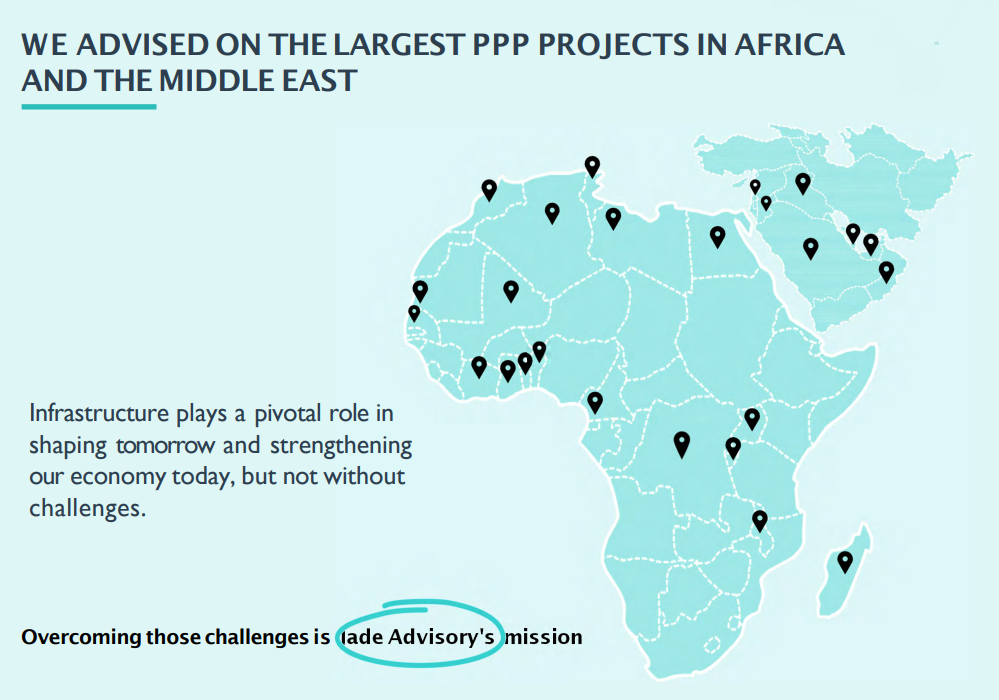
\includegraphics[width=0.9 \linewidth]{assets/jade-reg.png}
    \caption{Distribution of jade advisory projects in the MENA}
    \label{fig1}
\end{figure}

\subsection{Jade Advisory core team}
There are 5 people in the team who are experts in setting up projects that involve public and private partnerships in Africa and the Middle East. The different skills of its international team in strategy, consulting, and PPP services help them give advice that helps businesses grow and make more money. The senior team's skills in English, French, and Arabic help them communicate easily and understand different markets.
%Its dedicated team of five professionals has a proven track record in operationalizing PPP projects across Africa and the Middle East. The diverse expertise of its international team in strategy, consultancy and PPP services ensures it provide insights that drive business growth and profitability. its senior team's proficiency in English, French, and Arabic facilitates seamless communication and understanding across various markets.
\begin{enumerate}
    \item \textbf{Name}: Khaled Amri \\
    \textbf{Role}: Managing Director \\
    \textbf{Background}: Creator of Jade Advisory. Khaled has over 21 years of experience working as a PPP specialist in Europe, the Middle East, and Africa. He used to work at Ernst and Young MENA as a Director in the PPP Team, the French Railway Authority on High Speed Rail PPPs, Commerbank, and General Company Investment Bank in Paris. He has a Master's degree in civil engineering and another Master's in Project Finance and Structured Finance from Ecole of Ponts ParisTech.%Founder of Jade Advisory. Khaled is a PPP specialist with an exeperience of over 21 years in Europe, the Middle East and Africa. He previously worked at Ernst and Young MENA as a Director within the PPP Team, the French Railway Authority on High Speed Rail PPPs, Commerbank and General Company Investment Bank in Paris. He holds a Master's degree in civil engineering and a second Master's in Project Finance and Structured Finance from Ecole des Ponts ParisTech.
    \item \textbf{Name}: Mohamed Amine Sdiri\\
    \textbf{Role}: Director \\
    \textbf{Background}: Mohamed Amine has worked as a Civil Engineer for 11 years in different areas such as international development, government projects, public-private partnerships, and transportation systems. He has a postgraduate diploma in management and international relations from Sciences Po Paris and a Master of Engineering from ENIT Tunisia .%Mohamed Amine is a Civil Engineer with over 11 years of diversified experiences in international development, public sector, PPPs and transport infrastructures. He holds a postgraduate diploma in management and international relations from Sciences Po Paris and a Master of Engineering from ENIT (Tunisia).

    \item \textbf{Name}: Farouk Bouhafs \\
    \textbf{Role}: Senior Consultant \\
    \textbf{Background}: Farouk has a master's degree in Management and Strategy from IHEC Carthage in Tunisia. He has more than 5 years of professional experience in development projects, public private partnerships, project finance and infrastructure advisory. Before joining Jade, Farouk worked as project manager for a consulting company that focuses on helping countries grow and develop.%Farouk holds a master degree in Management and Strategy from IHEC Carthage (Tunisia). He has more than 5 years of professional experience in development projects, public-private partnerships, project finance and infrastructure advisory. Before joining Jade, Farouk worked as project manager for a consulting company specializing in international development.

    \item \textbf{Name}: Houyem Rais \\
    \textbf{Role}: Consultant \\
    \textbf{Background}: Houyem has a bachelor's degree in business administration, with a focus on finance and business analysis, from Tunis Business School TBS . She is a Thomas Jefferson scholarship program (TJSP) alumnus. She started working at Jade Advisory in January 2023.%Houyem holds a bachelor's degree in business administration (Major: Finance, Minor: Business Analysis) from Tunis Business School (TBS). She is a Thomas Jefferson scholarship program (TJSP) alumnus. She joined Jade Advisory in January 2023.

    \item \textbf{Name}: Mohamed Chiheb Tlili \\
    \textbf{Role}: Associate Consultant \\
    \textbf{Background}: Chiheb holds a Master's degree in finance from Mediterranean School of Business. He recently started working as an Associate Consultant at Jade Advisory.%Chiheb holds a Master's degree in finance from the Mediterranean School of Business. He recently joined Jade Advisory as an Associate Consultant. 
    
    
\end{enumerate}



\subsection{Sectors of activity}
Jade Advisory mainly focuses on different areas, as shown in the following \textbf{Figure \ref{fig2} } .
\begin{figure}[H]
    \centering
    
\includegraphics[width=0.9 \linewidth]{assets/jade-sectors.png}
    \caption{Jade Advisory working areas}
    \label{fig2}
\end{figure}
\subsubsection*{Infrastructure Advisory in the transport sector}
%Jade Advisory specialize in delivering comprehensive infrastructure advisory services tailored to the dynamic transport sector. Its expertise serves a diverse clientele, including Private Investors, Governments, International Financial Institutions and Development Agencies. This includes transportation economics, toll management solutions, lifecycle management as well as commercial advisory to physical asset investors, owners, developers and contractors over the project lifecycle, we can see this in table 1.1.
Jade Advisory focuses on providing expert advice on infrastructure for the transport industry. Its
serves many different types of clients, such as Private Investors, Governments, International Financial Institutions, and Development Agencies. This includes transportation economics, toll management solutions, lifecycle management, and commercial advisory for people who invest, own, develop, and build physical assets throughout a project's lifespan, as shown in \textbf{Table \ref{tab0} } .
\begin{table}[H]
    \centering
    \caption{Transport Sector Solutions}
    \label{tab0}
    \begin{tabular}{|>{\raggedright\arraybackslash}p{4.5cm}|>{\raggedright\arraybackslash}p{4.5cm}|>{\raggedright\arraybackslash}p{4.5cm}|}
        \hline
        \rowcolor[gray]{0.8}
        \textbf{Transportation Economics} & \textbf{Toll Management Solutions} & \textbf{Infrastructure Project Lifecycle Management} \\ \hline
        \begin{itemize}
            \item Optimizing financial viability and return on investment (ROI).
            \item Identifying financial risks associated with transportation initiatives and developing tailored mitigation strategies.
            \item Financial modeling and analysis that empowers clients to make well-informed decisions regarding their transportation projects.
        \end{itemize}
        &
        \begin{itemize}
            \item Implementing solutions that maximize revenue collection and financial performance for toll-based transportation projects.
            \item Streamlining toll collection systems and processes, enhancing operational efficiency and reducing costs.
            \item Fostering profitable collaboration between public and private stakeholders.
        \end{itemize}
        &
        \begin{itemize}
            \item Crafting detailed financial roadmaps that guide clients through every stage of infrastructure projects, from inception to completion.
            \item Aligning financing strategies with project milestones, ensuring that financial resources are allocated efficiently.
            \item Developing proactive risk mitigation plans, safeguarding the financial health of infrastructure projects and enhancing investor confidence.
        \end{itemize} \\ \hline
    \end{tabular}
\end{table}




\subsubsection*{Infrastructure Advisory in the water sector}
Jade Advisory uses its knowledge to help with water management. They provide specialized advice on infrastructure to Private Investors, Governments, and Development Agencies. Their main areas of work involve making sure water is used in the best way possible, including finding ways to make seawater usable and managing waste water. We also make sure that our projects are financially sound and that we use water resources efficiently. This can be seen in \textbf{Table \ref{tab1} }.%Jade Advisory leverages its expertise to address the critical water management sector, offering specialized infrastructure advisory services to Private Investors, Governments and Development Agencies. Our focus encompasses water supply optimization, desalination solutions and wastewater management, ensuring financial sustainability and efficient water resource utilization, we can see this in table 1.2.
\begin{table}[h]
    \centering
    \caption{Water Sector Solutions}
    \label{tab1}
    \begin{tabular}{|>{\raggedright\arraybackslash}p{4.5cm}|>{\raggedright\arraybackslash}p{4.5cm}|>{\raggedright\arraybackslash}p{4.5cm}|}
        \hline
        \rowcolor[gray]{0.8}
        \textbf{Water Supply Optimization} & \textbf{Desalination Solutions} & \textbf{Wastewater Management} \\ \hline
        \begin{itemize}
            \item Evaluating water supply projects for economic viability, ensuring sustainable access to clean water for communities
            \item Identifying financial risks in water supply initiatives and developing tailored mitigation strategies
            \item Provide financial modeling and analysis to support innovative water management strategies, optimizing water supply systems for long-term success.
        \end{itemize}
        &
        \begin{itemize}
            \item Implementing cost-effective desalination solutions, providing access to freshwater resources in water-scarce regions.
            \item Streamlining desalination operations, reducing costs and enhancing financial sustainability.
            \item Fostering collaboration between public and private stakeholders to achieve financial success while ensuring reliable desalination services
        \end{itemize}
        &
        \begin{itemize}
            \item Evaluating the financial viability of wastewater management projects, ensuring they meet economic and environmental goals.
            \item Developing financing strategies tailored to the unique needs of wastewater management initiatives.
            \item Promote projects that achieve financial sustainability while advancing responsible wastewater management and environmental protection.
        \end{itemize} \\ \hline
    \end{tabular}
\end{table}

\subsubsection*{Infrastructure Advisory in the waste management sector} 
Jade Advisory helps with waste management. They give advice to different kinds of clients, like private investors, governments, financial institutions, and development agencies. This covers turning waste into resources, following environmental rules, being sustainable, and managing finances during projects. We can find more information in \textbf{Table \ref{tab2} }.
%Jade Advisory extends its expertise to the waste management sector, offering tailored infrastructure advisory services to a wide-ranging client base, encompassing Private Investors, Governments, International Financial Institutions, and Development Agencies. This encompasses waste-to-resource transformation, environmental compliance and sustainability, as well as comprehensive financial project lifecycle management, we can see this in table 1.3.

\begin{table}[H]
    \centering
    \caption{Waste Management Sector Solutions}
    \label{tab2}
    \begin{tabular}{|>{\raggedright\arraybackslash}p{4.5cm}|>{\raggedright\arraybackslash}p{4.5cm}|>{\raggedright\arraybackslash}p{4.5cm}|}
        \hline
        \rowcolor[gray]{0.8}
        \textbf{Waste-to-Resource Transformation} & \textbf{Environmental Compliance and Sustainability} & \textbf{Infrastructure Project Lifecycle Management} \\ \hline
        \begin{itemize}
            \item Optimizing waste management projects for maximum resource recovery.
            \item Identifying opportunities for cost-effective waste-to-resource transformation, enhancing financial performance for both public and private stakeholders
            \item Providing innovative strategies to convert waste into valuable resources, contributing to a circular economy and financial sustainability.
        \end{itemize}
        &
        \begin{itemize}
            \item Optimizing waste management projects for maximum resource recovery.
            \item Identifying opportunities for costeffective waste-to-resource transformation, enhancing financiaperformance for both public and privatstakeholders
            \item Providing innovative strategies to convert waste into valuable resources, contributing to a circular economy  financial sustainability
        \end{itemize}
        &
        \begin{itemize}
            \item Navigating complex environmental regulations and ensuring compliance, mitigating financial risks associated with non-compliance.
            \item Promoting environmentally sustainable waste management practices that reduce long-term financial liabilities and enhance environmental stewardship
            \item Financial modelling and analysis that aligns waste management projects with environmental sustainability
        \end{itemize} \\ \hline
    \end{tabular}
\end{table}

\subsubsection*{Infrastructure Advisory in the social infrastructures sector}
Jade Advisory uses their knowledge to help with important social projects. They offer advice to both private investors and public organizations about infrastructure. This involves making healthcare, schools, and cultural centers better, and improving the community. It helps society grow and be financially stable.
%Jade Advisory brings its expertise to the critical social infrastructure sector, tailoring infrastructure advisory services to Private Investors and Public Entities. This encompasses healthcare infrastructure excellence, educational facilities enhancement, and the development of cultural and community centers, enriching the fabric of society and fostering financial sustainability.



\subsubsection*{Infrastructure Advisory in the agriculture}
%Jade Advisory provides its expertise to the thriving agriculture sector, offering tailored infrastructure advisory services that benefit Private Investors, Farmers, Smallholders, Rural Communities, Governmental Bodies and Development Agencies. This encompasses agroparks development, agribusiness and irrigation, and sustainable rural development, fostering financial sustainability and agricultural excellence.
Jade Advisory helps the growing agriculture industry by giving advice on infrastructure. This helps Private Investors, Farmers, Smallholders, Rural Communities, Government Bodies, and Development Agencies. This includes the growth of agroparks, agribusiness, irrigation, and rural development that helps farmers and communities become financially stable and excel in agriculture.

\section{Project presentation}
In this section, we will talk about current state, what's wrong with it, and suggest ways to make things better and help the business do well.
%In this section, we will outline the current state, critique it, and propose solutions to address challenges and improve enterprise performance.
\subsection{Study of the existing}
Public private partnerships PPPs have become very important in the global infrastructure sector. They help reduce costs and address economic challenges in areas like transportation and energy.
%Public-private partnerships (PPPs) have indeed emerged as indispensable options in the global infrastructure environment, offering promising solutions to lower infrastructure costs and overcome economic constraints in sectors such as transport , energy, and others. 
\vskip 0.5cm
However, using the traditional methods to see if PPP projects are possible can cause some problems. These methods can be tiring, costly, and rely too much on experts, old data, and basic financial models. They provide some useful information but may not be advanced enough to handle the complexity and uncertainty of infrastructure.
%However, traditional methods of feasibility assessment for PPP projects result in distinct inefficiencies. These methods are often laborious, expensive, rely too heavily on expert judgment, historical data, and simple financial models Despite providing some valuable insight, often these methods lack the necessary sophistication required to effectively deal with the complexity and uncertainty of infrastructure.
\vskip 0.5cm
Additionally, as the number of project files and documents increased, organizations like Jade Advisory realized they need for better ways to work together and manage resources. That's why they started using platforms like OneDrive for easier teamwork and improved management. Jade Advisory decided to use ChatGPT as an AI assistant in their work, which can help them better conduct studies and manage project documents. This accreditation involves tasks like reviewing documents, feasibility studies, and asking for advice from experts.
%Additionally, as the volume of project files and documents increased, organizations such as Jade Advisory recognized the need for advanced collaboration and resource management solutions and therefore moved to platforms such as OneDrive in order with easier teamwork and better management. However, Jade Advisory chose to incorporate ChatGPT as an AI assistant in their workflow,which could strengthen their ability to conduct feasibility studies and manage project documentation more efficiently. This accreditation includes activities, including review of documents, feasibility studies, and seeking expert recommendations.
\subsection{criticism of the existing}
% Jade advisory think highly of data privacy, due to sensitive and proprietary information included in its project files .Therefore ,OneDrive isn't a good choice because it is developed and managed by Microsoft. Even if your data is encrypted, Microsoft can get access to it.Otherwise ,communicating documents with chatgpt not only could present  confidentiality issues but also its very slow in term of response speed while dealing with multi-documents on account of the documents curation.
% It's also important to consider the context in which ChatGPT is used and to verify the information it provides through independent sources when necessary, especially in situations where the accuracy and reliability of the information are paramount.
% Jade Advisory lacks a dedicated engineering team or prior expertise. Consequently, ChatGPT might pose a risk by relying on independent sources for information, potentially leading to distractions in its operations, especially in situations where the accuracy and reliability of the information are paramount.

Although public private partnerships PPPs offer promising solutions for building infrastructure, traditional feasibility study methods have many criticisms because they are inefficient and have limitations.
%Although public-private partnerships (PPPs) offer promising solutions in terms of infrastructure development, conventional feasibility study methods face several important criticisms stems from the inefficiencies and various limitations of the current methods.
\vskip 0.5cm
First, using old methods to do feasibility studies with lots of manual work is really hard. These methods are usually slow, require lots of work, and are prone to mistakes. They also cause delays and inefficiencies in decision-making. Relying on expert opinions can lead to subjective and biased results, instead of objective and thorough analysis.
%First, the reliance on traditional methods for conducting feasibility studies, characterized by manual work, presents major challenges. These methods are often time-consuming, labour-intensive and error-prone, in addition to delays and inefficiencies in decision-making processes, their reliance on expert judgment as the primary source of insight encourages subjectivity and bias, and destroys objectivity and robust analysis.
\vskip 0.5cm
Besides, traditional approaches prioritize economic and neglect other important things like social impact, environmental sustainability, and technical development. This limited perspective hinders a full understanding of project feasibility and overlooks potential risks and opportunities that may come from non financial factors.
%Besides, traditional approaches prioritize economic considerations while ignoring other important feasibility considerations, such as social and economic impact, environmental sustainability, and technical development This narrow view limits the broader understanding of project feasibility and ignores potential risks and opportunities that may arise from non-financial factors.
\vskip 0.5cm
Howerver, The absence of automation for everyday tasks like creating reports still causes problems with projects and makes stakeholders less productive.
%However, the lack of automation for common tasks such as report generation continues to contribute to inefficient projects and decrease productivity for stakeholders.
\vskip 0.5cm
Also, ChatGPT's lack of user interaction makes it less efficient and slows down decision-making. Participants may have trouble understanding and using the information given by the AI assistant, which could decrease their effectiveness.
%Furthermore, ChatGPT’s limited user interactivity hinders efficiency and decision making. Participants may have difficulty accessing and interpreting the insights provided by the AI assistant, limiting their ability to fully utilize them.
\vskip 0.5cm
Moreover, the limited access to ChatGPT makes it hard for people with technical skills or disabilities to fully take part in the study. However, the way ChatGPT deals with issues relating to the project, wich is careful and respectful of privacy concerns. Without following strict safety rules, people involved may hesitate to work with AI, which can make the feasibility study process less trustworthy and efficient.
%Furthermore, the limited accessibility of ChatGPT creates barriers for participants with technical skills or disabilities, preventing them from fully participating in the feasibility study process. Nevertheless, how ChatGPT handles related to the project is sensitive to privacy and confidentiality concerns arise. Without strict safety protocols, stakeholders may be reluctant to interact with AI, undermining the integrity and effectiveness of the feasibility study process.
\vskip 0.5cm
In summary, current methods for assessing the feasibility of PPPs have problems like being inefficient, subjective, and only focusing on economic factors. These limits, with difficulties linked to combining data, automating tasks, engaging users, making things easy to access, and protecting privacy. They emphasize the need for a big change in how we make decisions, moving towards more thorough and objective methods.
%In summary, existing feasibility assessment methods in PPPs suffer from inefficiencies, subjectivity, and narrow attention to economic considerations. These constraints, with challenges related to data integration, automation, user interaction, accessibility and privacy. They highlight the necessity for a paradigm shift towards more comprehensive, objective and integrated approaches to ensure robust decision-making.
\vskip 0.5cm
The \textbf{Table \ref{tab5} } shows some possible problems with OneDrive and ChatGPT.
\begin{table}[h!]
    \begin{center}
    \caption{oneDrive and ChatGPT cons}
    \label{tab5}
    \begin{tabular}{{|c|p{0.6\textwidth}|}}
    \hline
     \rowcolor[gray]{0.8}\bfseries Software & \bfseries Cons \\
    \hline
    \raisebox{-1\height}{
\includegraphics[scale = 0.3]{assets/oneDrive.png}} & 
    \begin{itemize}
        \item Weak data privacy.
        \item Data Vulnerability.
        \item Synchronization Limits.
        \item Limited Backup Functionality.
        \end{itemize}\\
     \hline
    \raisebox{-0.9\height}{
\includegraphics[scale = 0.2]{assets/chatgpt.png}} & 
    \begin{itemize}
        \item Provides Inaccurate Information.
        \item Biased Responses.
        \item Limited Knowledge.
        \end{itemize}\\
     \hline
  \end{tabular}
  \end{center}
  
\end{table}


\subsection{Proposed soultion}
To overcome problems with current methods offeasibility assessment in PPPs, we suggest new solutions that use cutting-edge technology to make decisions faster, fairer, and more effective.
%To address the limitations and criticisms of existing approaches to feasibility assessment in PPPs, we propose comprehensive and innovative solutions that use and drive advanced technologies key factors combine to increase efficiency, objectivity and effectiveness in decision-making processes.
\vskip 0.5cm
First of all, Our solution focuses on making it easy for Chat assistance and documents to work together smoothly, allowing data to be exchanged and synchronized seamlessly. This integration will take off the need for people to manually use ChatGPT, make the feasibility study process easier, and boost overall performance. besides, a strong data integration process will be put in place to protect the privacy and confidentiality of important project information.
%First of all, our solution prioritizes seamless integration between Chat assistance and documents, enabling seamless data exchange and synchronization. This integration will eliminate manual interaction with the ChatGPT alternative, simplify the feasibility study process and improve overall performance. Additionally, a robust data integration process will be implemented to ensure the privacy and confidentiality of critical project information.
\vskip 0.5cm
Secondly, we will use technology to make tasks like making reports easier by automating them. Using machine learning algorithms, our solution will help automate comparing reports, saving time and reducing mistakes. This automation will increase productivity so that stakeholders can focus on important tasks that need human skill.
%Secondly, we will add automation capabilities to streamline common tasks such as report generation. Using machine learning algorithms, our solution will automate comparative reporting, reducing manual effort, reducing risk of errors This automation will drive productivity higher to enable stakeholders to focus on higher-value tasks that require human expertise.
\vskip 0.5cm
Thirdly, our solution will have an easy-to-use interface that works well with ChatGPT alternative. We focus on making it easy for people to chat with our assistance, ask questions, and interpreting insights. This better connection will bring together users and make sure that participants can fully utilize the power of AI.
%Thirdly, our solution will provide an intuitive and user-friendly interface, facilitating seamless integration with ChatGPT alternative. We prioritize interactive features that enable participants to effortlessly interact with chat assistance, asking questions, and interpreting insights. This improved connectivity will integrate users and ensure participants can cover the full potential of AI.
\vskip 0.5cm
Our goal is to make sure that our solutions can be used by all people with different skills and abilities. We will give training and support materials to help everyone effectively use the solution.
%Fourthly, we are committed to ensuring that our solutions are accessible to stakeholders with a range of technical skills and abilities. In addition, we will provide comprehensive training and support materials to empower all stakeholders to effectively implement the solution.
\vskip 0.5cm
Our solution will also have strong privacy and confidentiality protections to keep sensitive business data safe. Use encryption, access controls, and audit trails to keep data safe and secure during the analysis process. Make sure to focus on protecting data. Build trust with stakeholders to successfully implement the solution.
%Fifthly, our solution will incorporate robust privacy and confidentiality measures to protect sensitive business data. Implement encryption protocols, access controls and audit trails to ensure data integrity and security throughout the feasibility analysis process Prioritize data security Develop trust and confidence among stakeholders, and to enable the peaceful implementation of the solution.
\vskip 0.5cm
%In summary, our proposed solution provides a holistic approach to address the limitations and criticisms of existing approaches to research in PPPs. By prioritizing data integration, automation, user interactivity, accessibility and privacy, we aim to revolutionize the feasibility analysis process, empowering stakeholders to make decisions.
In summary, our idea offers a complete way to fix the problems with current methods in PPPs.
By focusing on combining data, automation, user engagement, accessibility, and privacy, we want to change how feasibility analysis works and help stakeholders make better choices.
\section{Conclusion}
%We have presented the host company, detailing the core team members and main sectors of activity. Additionally, we have included the presentation of our project, in which we have addressed the existing situation that has been criticized, and then proposed our project solution. Finally, in the next chapter, we will analyze the project's needs.
We have introduced the host company, highlighting the key team members and main areas of work. Moreover, we have included a presentation of our project, in which we have discussed the current issues that have received criticism and then put forward our proposed solution. Finally, in the next chapter, we will look at the project's requirements.
\chapter{Needs Analysis}

\section{Introduction}
The success of any work depends on the quality of its start. As a first step in our project, it is necessary to analyze the system requirements, which is the objective of this chapter.
\vskip 0.5cm
In the first part, we will study the needs and present the goals of our project by specifying the functional and non-functional requirements, as well as the external units that interact with the system. In the second part, we will present the development tools that allowed us to carry out this project and the working method used to prepare this report. Finally, we will focus on defining the use case diagram..

\section{Functional needs}
To ensure that our solution meets the expectations of users, it is crucial to identify all the functional requirements that the system must fulfill. These requirements, which are presented in use case diagram in \textbf{Figure \ref{fig:usecase}}, define the features that the system must provide to the user. Therefore, before starting the development of PPP AI assistance , it is imperative to ensure that all functional requirements have been clearly defined and documented.
\begin{itemize}
    \item \textbf{Chat With Private Document:} This feature allows users to have private conversations with the AI assistant, ChatGPT alternative, while securely sharing and receiving private documents. Users can interact with document assistance in real time for help, ask questions and receive personalized recommendations, all in a secure and private environment.
    \item \textbf{Feasibility Document Generation:} This functionality led to viable generation for public-private partnership (PPP) projects. Using pre-defined machine learning models and parameters, the system analyses project data, financial metrics, and other relevant data to generate detailed feasibility reports. Users can customize document content and structure to their specific needs, simplifying document organization and ensuring accuracy and consistency in reports.
    \item \textbf{Authentication:} The authentication process provides users with authorized access, ensuring privacy and data integrity is protected by establishing a secure framework for real-time communication. This provides easy access private conversations and sharing of secure documents between stakeholders. Users authenticate themselves for traceability, control and personalization purposes.
\end{itemize}

\begin{figure}[h]
    \centering
    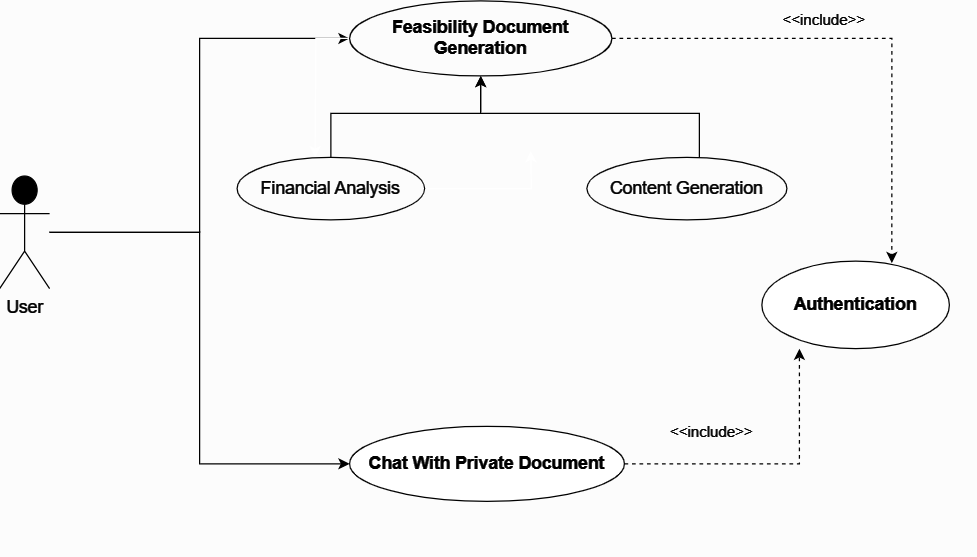
\includegraphics[width=1 \linewidth]{assets/diag.png}
    \caption{Use case diagram}
    \label{fig:usecase}
\end{figure}

\section{Technical specification}
\subsection{Non-functionnal needs}
The system must address non-functional requirements that are not essential to its operation but crucial for ensuring service quality and smooth system functioning. Non-functional requirements are internal system requirements essential for achieving our objective. To achieve this, the following requirements must be met:
\begin{itemize}
    \item \textbf{ergonomics}: Our product must feature an easy-to-use, user-friendly interface that optimizes interaction between humans and the system, even for inexperienced users. Users should be able to navigate the system effortlessly and access its functionalities without requiring any technical training.
    \item  \textbf{performance}:  Its crucial that our system must be optimized for efficiency to ensure fast response times and efficient handling of requests by reducing latency qnd improving resource utilization
    \item \textbf{Reliability}: The system should be highly reliable, with minimal downtime and disruption.The AI assistance should possess contextual awareness of the PPP project and deliver precise results consistently. 
    \item \textbf{Scalability}: The system should be scalable, capable of efficiently adapting to future demands and user growth without compromising performance.
    \item \textbf{Security }: Our system prioritizes robust security measures to safeguard sensitive data, prevent unauthorized access, and maintain compliance with industry regulations.  
\end{itemize}
\subsection{Hardware environment}
In total, our hardware environment consists of two laptops, as shown in the following \textbf{Table \ref{tab:HWE}}.

\begin{table}[h!]
\begin{center}
\caption{Hardware environment}
\label{tab:HWE}
\begin{tabular}{{|c|p{5cm}|p{5cm}|}}
\hline
\rowcolor[gray]{0.8} \bfseries{Specification} & \bfseries{HP Pavilion Gaming Laptop} & \textbf{Dell laptop} \\ 
\textbf{Operating System}       & Microsoft Windows 11 Famille Unilingue & Not specified \\
\hline
\textbf{CPU}     & Intel Core i5-10300H (2.50 GHz, 4 cores, 8 logical processors) & Intel Core \\ 
\hline
\textbf{RAM}     & 32 GB total physical memory + 36.5 GB virtual memory & Not specified \\ 
\hline
\textbf{GPU}     & NVIDIA GeForce GTX 1650 Ti & MX330 \\ 
\hline
\textbf{Storage} & 500GB & 500GB \\ 
\hline 
\end{tabular}
\end{center}
\end{table}

\subsection{Software environment}
Our adopted software are Python, LangChain, Ollama, PostgreSQL, Docker, Streamlit and LangFuse, as shown in the following table 2.2.


\begin{longtable}{|p{4cm}|p{10cm}|}
    \caption{Software environment}\label{tab6} \\
    \hline
    \rowcolor[gray]{0.8} \textbf{Software} & \textbf{Description} \\
    \hline 
    \endfirsthead

    \hline
    \rowcolor[gray]{0.8} \textbf{Software} & \textbf{Description} \\
    \endhead

    \hline 
    \multicolumn{2}{|r|}{\footnotesize Continued on next page} \\
    \hline
    \endfoot

    \hline
    \endlastfoot

    \raisebox{-1.55\height}{
\includegraphics[scale=0.2]{assets/python.jpg}} & 
    Python is a high-level programming language that is widely known for being beginner-friendly with an active community contributing to open-source projects. \\
    \hline
    \raisebox{-1.15\height}{
\includegraphics[scale=0.35]{assets/postgres.png}} & 
    PostgreSQL is an open-source relational database known for robustness and versatility. \\
    \hline
    \raisebox{-0.7\height}{
\includegraphics[scale=0.2]{assets/ollama.png}} & 
    Ollama allows you to run open-source large language models locally. \\
    \hline
    \raisebox{-1.5\height}{
\includegraphics[scale=0.2]{assets/langfuse.png}} & 
    LangFuse is an open-source platform designed for engineering with Large Language Models (LLMs). \\
    \hline
    \raisebox{-1.25\height}{
\includegraphics[scale=0.05]{assets/streamlit.png}} & 
    Streamlit simplifies data science app creation by focusing on Python skills instead of web development. \\
    \hline
    \raisebox{-0.9\height}{
\includegraphics[scale=0.03]{assets/Docker-Logo.png}} & 
    Docker is a platform as a service product that uses OS-level virtualization to deliver software in containers. \\
    \hline
\end{longtable}

    





\section{Conclusion}
In summary, we've addressed both functional and non-functional needs, ensuring user satisfaction and system performance. Then we have discussed the Hardware and software environment considerations in order to satisfy the non-functional requirements. In the next chapter, we will delve into exploring the landscape of artificial intelligence.





\chapter{State of Artificial Intelligence }
%longtable for review

\section{Introduction}
%In this chapter, we delve into the foundation of our AI assistance, the large language model, which serves as the powerful engine of our system. Meanwhile, understanding the current state of artificial intelligence is imperative to harnessing its capabilities effectively. Therefore, we explore the landscape of artificial intelligence in its current form to contextualize the development of our AI assistance.
In this chapter, we discuss the foundation of our AI assistance, the large language model, which is like the powerful engine of our system. Meanwhile, it is very important to understand the current state of artificial intelligence in order to use its capabilities properly. Therefore, we explore the landscape of artificial intelligence in its current form to contextualize the development of our AI assistance. 
\section{Large language model (LLM)}
\subsection{Definition}
At its core, a large language model is a type of computer program that can understand and create human language using neural networks. The main job of a language model is to figure out the chances of a word coming next in a sentence. For instance, in the sentence "The sky is ......" the most common answer would be "blue". The model can guess the next word in a sentence by looking at a big collection of text. Basically, it learns to recognize patterns in the words. You get a pre-trained language model from this process
%At its core, a large language model is a type of machine learning model that can understand and generate human language via deep neural networks. The main job of a language model is to calculate the probability of a word following a given input in a sentence: for example, “The sky is .......” with the most likely answer being “blue”. The model is able to predict the next word in a sentence after being given a large text dataset (or corpus). Basically, it learns to recognize different patterns in the words. From this process, you get a pre-trained language model.
\vskip 0.5cm
The following \textbf{Figure \ref{fig:artificial-intelligence}} \cite{w9} illustrates the layers within the field of Artificial Intelligence.
\begin{figure}[H]
    \label{fig:artificial-intelligence}
    \centering
    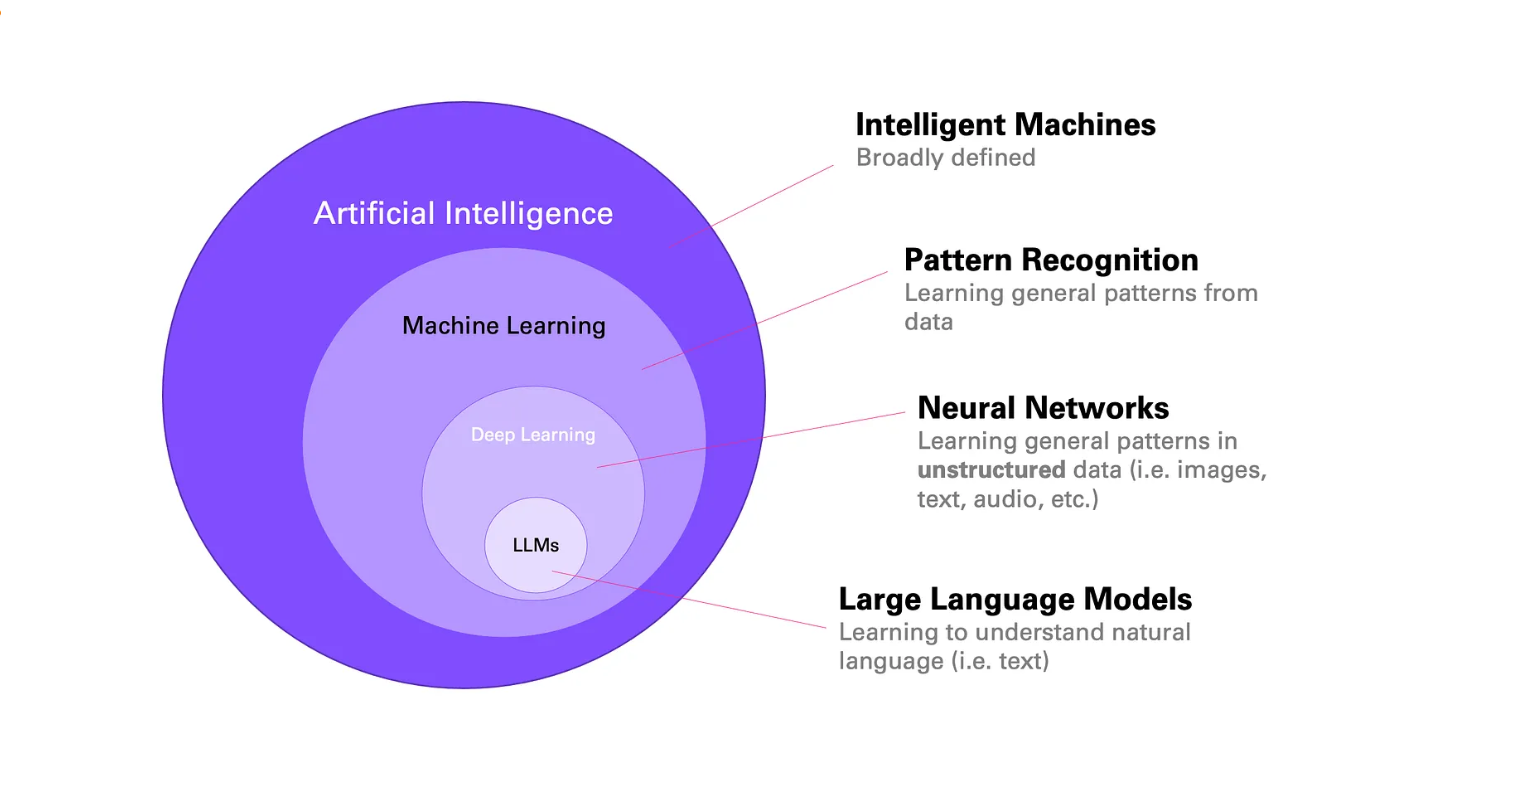
\includegraphics[width=0.83 \linewidth]{assets/art.png}
    \caption{The field of Artificial Intelligence in layers}
\end{figure}

\subsection{History}
%Through the 1990s and early 2000s, the AI industry was focused on small-scale applications and pipelines that were less computationally complex and time-intensive as shows the following figure 3.2 \cite{w10}. Let’s briefly look at the history of LLMs.
During the 1990s and early 2000s, the AI industry mostly worked on small projects that were not too complicated or time-consuming. This can be seen in \textbf{Figure \ref{fig:llm_historic}} \cite{w10}. Let's quickly talk about the history of LLMs.
\begin{figure}[H]
    \label{fig:llm_historic}
    \centering
    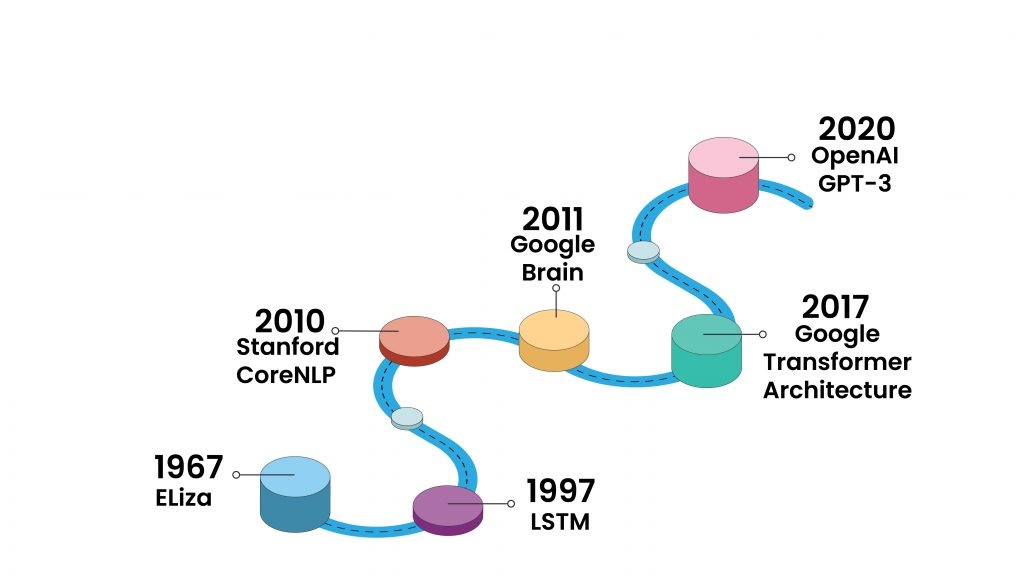
\includegraphics[width=1 \linewidth]{assets/llm_historic.jpeg}
    \caption{History of Large Language Models}
\end{figure}

When the ancients carefully recorded their knowledge on scrolls of papyrus and housed them in the legendary Library of Alexandria, they could not have even dreamed it possible that all that knowledge and more would be available at the fingertips of their descendants millenniums later. That’s the power and beauty of large language models. Not only can LLMs answer questions and solve complex problems, but they can also summarize huge volumes of work, as well as translate and derive context from various languages.
\vskip 0.5cm
The beginnings of big language models can be traced back to experiments with neural networks and neural information processing systems in the 1950s to help computers process and use natural language. Researchers at IBM and Georgetown University collaborated to develop a system that can translate phrases from Russian to English automatically. Research in machine translation started from there and gained a lot of recognition.
%The foundation of large language models can be traced back to experiments with neural networks and neural information processing systems that were conducted in the 1950s to allow computers to process natural language. Researchers at IBM and Georgetown University worked together to create a system that would be able to autoatically translate phrases from Russian to English. As a notable demonstration of machine translation, research in this field took off from there.
\vskip 0.5cm
The concept of LLMs started with Eliza, the first chatbot created by MIT researcher Joseph Weizenbaum in the 1960s. Eliza started the study of natural language processing NLP , laying the groundwork for advanced LLMs in the future. Then after about 30 years, in 1997, Long Short Term Memory LSTM networks were invented. Their arrival led to more advanced and sophisticated neural networks that could process larger amounts of data. Stanford's CoreNLP suite, launched in 2010, made it possible for developers to analyze feelings and identify entities in text.
%The idea of LLMs was first floated with the creation of Eliza in the 1960s: it was the world’s first chatbot, designed by MIT researcher Joseph Weizenbaum. Eliza marked the beginning of research into natural language processing (NLP), providing the foundation for future, more complex LLMs. Then almost 30+ years later, in 1997, Long Short-Term Memory (LSTM) networks came into existence. Their advent resulted in deeper and more complex neural networks that could handle greater amounts of data. Stanford’s CoreNLP suite, introduced in 2010, was the next stage of growth allowing developers to perform sentiment analysis and named entity recognition.
\vskip 0.5cm

In 2011, a smaller Google Brain with better features like word embeddings helped NLP systems understand context better. This was a big moment, with models becoming popular in 2017. Think, which is short for Generative Pre-trained Transformer, can create or "decode" new writing. Another example is BERT - Bidirectional Encoder Representations from Transformers. Wich analyze input text to make predictions or categorize it based on encoder parts.
%Subsequently, in 2011, a smaller version of Google Brain appeared with advanced features such as word embeddings, which enabled NLP systems to gain a clearer understanding of context. This was a significant turning point, with transformer models bursting onto the scene in 2017. Think GPT, which stands for Generative Pre-trained Transformer, has the ability to generate or “decode” new text. Another example is BERT – Bidirectional Encoder Representations from Transformers. BERT can predict or classify input text based on encoder components.
\vskip 0.5cm
%From 2018 onward, researchers focused on building increasingly larger models. It was in 2019 that researchers from Google introduced BERT, the two-directional, 340-million parameter model (the third largest model of its kind) that could determine context allowing it to adapt to various tasks. By pre-training BERT on a wide variety of unstructured data via self-supervised learning, the model was able to understand the relationships between words. In no time at all, BERT became the go-to tool for natural language processing tasks. In fact, it was BERT that was behind every English-based query administered via Google Search.
From 2018 onwards, researchers concentrated on creating bigger and bigger models. In 2019, Google researchers introduced BERT, a large model with 340 million parameters. It can understand context in both directions and can be used for different tasks. By training BERT on many different types of data without supervision, the model learned the relationships between words. BERT quickly became the top choice for tasks involving understanding and using human language. Actually, it was BERT that was responsible for every English query on Google Search.
\subsection{Types of Large Language Models (LLM)}
LLMs can be divided into three types pre-training models, fine-tuning models, and multimodal models. Different options have different benefits, depending on what you want to achieve:
%LLMs can be broken down into three types: pre-training models, fine-tuning models, and multimodal models. Each has its own advantage, depending on the goal:
\vskip 0.5cm
\begin{itemize}
    \item \textbf{Pre-training models}: are trained on huge quantities of data, which helps them comprehend a broad range of language patterns and constructs. A plus is that a pre-trained model tends to be grammatically correct!
    \item \textbf{Fine-tuning models}: are pre-trained on a large dataset and afterward are fine-tuned on a smaller dataset for a specific task (use case). They’re particularly good for sentiment analysis, answering questions, and classifying text.
    \item \textbf{Multimodal models}: combine text with other modes, such as images or video, to create more advanced language models. They can produce text descriptions of images and vice versa.
\end{itemize}

\subsection{Phases of training Large Language Models (LLMs)}
Large language models go through three main stages: pre training, fine-tuning for specific tasks, and learning from feedback from humans, as shown in \textbf{Figure \ref{fig:phases-llm}}\cite{w11}.
%Large language models undergo three main phases: pre-training, instruction fine-tuning, and reinforcement learning from human feedback as shows the following figure 3.3 \cite{w11}
\begin{figure}[H]
    \label{fig:phases-llm}
    \centering
    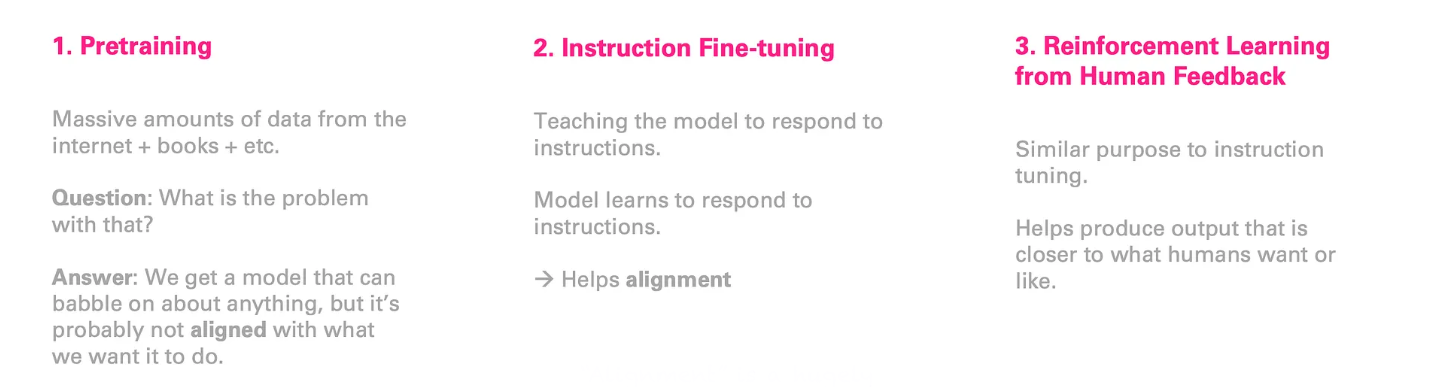
\includegraphics[width=0.9 \linewidth]{assets/gpt-phases.png}
    \caption{Phases of training LLMs}
\end{figure}

\subsubsection{Pre-training}
%stopped here !!!
This step needs a massive amount of data in order to train for predicting the next word. During this time, the model learns how to use language correctly and also gains knowledge about the world and develops new abilities.
%This stage requires massive amounts of data to learn to predict the next word. In that phase, the model learns not only to master the grammar and syntax of language, but it also acquires a great deal of knowledge about the world, and even some other emerging abilities
\vskip 0.5cm
%However, Pre-training a Large Language Model (LLM) primarily teaches it to ramble on about a topic, which can result in impressive output but poor performance in responding to specific inputs such as questions or instructions. This is because the LLM has not learned to be an assistant, but rather to complete input sequences. For example, when asked “What is your first name?”, a pre-trained LLM may respond with “What is your last name?” as it has been trained on many empty forms. The model struggles with following instructions because the structure of instruction followed by a response is not commonly seen in the training data. At this stage, the LLM is not aligned with human intentions, which is an important topic for LLMs. However, it can be taught to respond to instructions through further training. Despite initial difficulties, pre-trained LLMs are steerable, making it possible to teach them to follow instructions and align with human intentions.
However, training a large language model only teaches it to talk a lot about a topic, which can make it produce impressive results but not very good at answering specific questions or following instructions. The LLM has not learned to be an assistant, but instead to complete input sequences. For example, when someone asks "What is your first name?", a pre trained LLM might answer with "What is your last name?" because it has been trained on lots of empty forms. The model is having a hard time understanding instructions because it is not used to seeing a pattern where an instruction is given and then a response is expected. At this point, the LLM does not match up with what people want, which is a important concern for LLMs. However, it can learn to follow commands with more practice. Despite some challenges at first, pre-trained LLMs can be controlled and taught to follow directions and understand human goals.
\subsubsection{Instruction fine-tuning }
This is where instruction tuning comes in to adjust instructions. We use the pre-trained LLM with its current abilities and continue to predict one word at a time. This time, we only use high quality training data with instruction and response pairs.
%This is where instruction tuning comes in. We take the pre-trained LLM with its current abilities and do essentially what we did before — i.e., learn to predict one word at a time — but now we do this using only high-quality instruction and response pairs as our training data.
\vskip 0.5cm
%That way, the model un-learns to simply be a text completer and learns to become a helpful assistant that follows instructions and responds in a way that is aligned with the user’s intention. The size of this instruction dataset is typically a lot smaller than the pre-training set. This is because the high-quality instruction-response pairs are much more expensive to create as they are typically sourced from humans. This is very different from the inexpensive self-supervised labels we used in pre-training. This is why this stage is also called supervised instruction fine-tuning.
That way, the model un-learns to only complete sentences and learns to be a helpful assistant that follows directions and responds in a way that matches what the user wants. The size of this instruction dataset is usually much smaller than the pre-training set. high-quality instruction response pairs are very costly to make because they usually human annotated. This is very different from the cheap self-supervised labels we used in pre-training. This stage is also known as supervised instruction fine-tuning because of this reason.
%mdx
\subsubsection{Reinforcement Learning from Human Feedback (RLHF)}
At its core, RLHF uses human feedback to create a dataset of human preferences. This helps determine the reward function for a specific output. People can give feedback in many ways:
%On a basic level, RLHF implements human feedback to generate a human preferences dataset that ascertains the reward function for a desired outcome. Human feedback can be obtained in multiple ways:
\begin{itemize}
    \item \textbf{Order of preference}: People rank outputs in order of preference.
    \item \textbf{Demonstrations}: Humans write preferred answers to prompts.
    \item \textbf{Corrections}: Humans edit a model’s output to correct unfavorable behaviors.
    \item \textbf{Natural language input}: Humans provide descriptions or critiques of outputs in language. Once a reward model has been created, it’s used to train a baseline model with the help of reinforcement learning, which leverages the reward model to build a human values policy that the language model then uses to produce responses. ChatGPT is a good example of how a large language model uses RLHF to produce better, safer, and more engaging responses
    
\end{itemize}
%RLHF constitutes a major advancement in the realm of language models, providing a more controlled and reliable user experience. But there’s a tradeoff: RLHF introduces the biases of those who have contributed to the preference dataset used to train the reward model. So, while ChatGPT is geared toward helpful, honest, and safe answers, it’s still subject to the annotators’ interpretations of these answers. While RLHF improves consistency (which is great for the use of LLMs in search engines), it does so at the expense of creativity and diversity of ideas. There is still a lot to uncover in this area.
RLHF is a weighty step forward in language models, giving users a better and more reliable experience. However, there is a tradeoff, RLHF brings in the biases of the people who provided the data used to train the reward model. While ChatGPT aims to provide useful, honest, and self-confident answers, the way these answers are understood by the annotators can vary. RLHF improves consistency, but it reduces creativity and diversity of ideas. There is still a lot to discover in this area.
\subsection{Most Large Language Model Application}
%At first glance, LLMs can be used in any scenario where an organization needs to analyze, process, summarize, rewrite, edit, transcribe or extract insights from a dataset or input text. With adoption increasing, there are some practical applications of language models that appear to be promising.
At first look, LLMs can be used in any situation where a company needs to analyze, process,  summarize, rephrase, edit, transcribe or etract insights from a set of data or input text. With adoption increasing, there are some useful ways to use language models that seem to be very helpful.
\subsubsection{Translation With Language Models}
%One of the simplest practical applications for LLMs is to translate written texts. A user can enter text into a chatbot and ask it to translate into another language, and the solution will automatically begin translating the text.
One simple way to use LLMs is to change written words into a different language. A person can type in words to a chatbot and ask it to change them to a different language, and the chatbot will start translating the words automatically.
\subsubsection{Content Creation}
Another very common use for language models is creating content. LLMS allows people to create many different types of written content, like blogs, articles, short stories, summaries, scripts, questionnaires, surveys, and social media posts. The quality of these outputs relies on the provided in the initial prompt.
%Another increasingly common use case for language models is content creation. LLMS enables users to generate a range of written content from blogs and articles to short stories, summaries, scripts, questionnaires, surveys, and social media posts. The quality of these outputs depends on the details provided in the initial prompt.
\vskip 0.5cm
%If LLMs aren’t used to generate content directly, they can also be used to help with ideation. According to Hubspot, 33\% of marketers who use AI use it to generate ideas or inspiration for marketing content. The main value here, is that AI can speed up the content generation process. It’s worth noting that there are also tools like DALL-E, MidJourney, and Stable Diffusion that allow users to generate images based on a written prompt.
If LLMs are not used to create content, they can still be used to come up with new ideas. According to Hubspot, 33\% of marketers who use AI use it to come up with ideas or inspiration for marketing content. The key benefit here is that AI can make the process of creating content faster. There are tools like DALL E, MidJourney, and Stable Diffusion that let you make pictures from written prompts.
\subsubsection{Search}
Many users will first have experimented with generative AI as an alternative search tool. Users can ask a chatbot questions in natural language and will receive an instant response with insights and facts on potentially any topic.
\vskip 0.5cm
Using tools like Bard or ChatGPT to search for information gives you access to a lot of different information, but not all of it may be correct. 
%While using solutions like Bard or ChatGPT as a search tool provides access to a wide-range of information, it’s important to be aware that not all of this content is accurate.
\vskip 0.5cm
%Language models are prone to hallucination, and have a tendency to invent facts and figures. For this reason, it’s a good idea for users to double-check any factual information presented by LLMs so they can avoid being misled by misinformation.
Language models often make mistakes and can come up with false information. It is important for users to verify any facts shared by LLMs to avoid being misled by misinformation.
\subsubsection{Detecting and Preventing Cyber Attacks}
Another interesting use of language models in cybersecurity is identifying cyberattacks. LLMs are able to analyze big sets of data from a company's network and can detect patterns that show a harmful cyber attack and send a warning.
%Another interesting cybersecurity use case for language models is detecting cyberattacks. This is because LLMs have the ability to process large data sets collected throughout an enterprise network and can spot patterns that indicate a malicious cyber attack and generate an alert.
\vskip 0.5cm
So far, some companies are testing new technology to find and stop cybersecurity threats. For instance, earlier this year SentinelOne introduced a solution driven by LLM that can automatically search for threats and start automated responses of malicious activity.
%So far a number of cybersecurity vendors have begun experimenting with the technology for threat detection. For example, early this year SentinelOne released an LLM-driven solution that can automatically hunt for threats and initiate automated responses to malicious activity.
\vskip 0.5cm
%Another approach demonstrated by Microsoft Security Copilot, allows users to scan their environments for known vulnerabilities and exploits, and can generate reports on potential security events in minutes to equip human defenders to respond.
Another way shown by Microsoft Security Copilot, lets users check their systems for known weaknesses and attacks, and can create reports about possible security issues in a few minutes so that people can react quickly.
\subsubsection{Code Development}
Generative AI tools can create both natural language and code in languages like JavaScript, Python, PHP, Java, and C\#.
%Generative AI tools not only have the ability to generate natural language, but can generate code in languages like JavaScript, Python, PHP, Java, and C\#.
\vskip 0.5cm
\textsc{The language models can help non-technical users  to create simple code. Can write basic code for simple projects, but has difficulties with larger and more complex tasks  that are bigger in scope and scale.}
\vskip 0.5cm
%Thus programmers should double-check code for functionality and security issues during development to avoid disruption post-deployment. They can also be used to help debug existing code or even generate accompanying documentation so that users don’t have to spend time doing it manually.
Programmers need to carefully review their code for any problems with how it works or how secure it is before they finish working on it. This will help prevent any issues from happening after the code is in use. They can also be used to help fix problems in code or create documentation automatically, saving users time.
\subsection{Large Language Model tools}
large language models like LlaMA have various versions, such as llama2 7b, llama2 13b, and llama2 70b. These versions reflect the model’s size and capacity, with larger models having more parameters and being able to handle more complex tasks. The purpose of versioning is to offer different sizes and capabilities of the model to fit different needs and uses. For instance, a small model like llama2 7b could work well for a chatbot, while a larger model like llama2 70b might be better for generating content. Versioning allows developers to pick the best model for their needs, balancing resources and requirements.
%Large language models, such as LlaMA, have different versions, including llama2-7b, llama2-13b, and llama2-70b. These versions reflect the model’s size and capacity, with larger models having more parameters and being able to handle more complex tasks. The goal of versioning is to provide different sizes and capacities of the model to suit various applications and use cases. For example, a smaller model like llama2-7b may be suitable for a chatbot application, while a larger model like llama2-70b may be more appropriate for a content generation task. Versioning allows developers to choose the best model for their specific needs, balancing computational resources and task requirements.
\subsubsection{Open-source LLM Models}


\begin{longtable}{|>{\centering\arraybackslash}p{2.5cm}|>{\centering\arraybackslash}p{2cm}|>{\centering\arraybackslash}p{4cm}|>{\centering\arraybackslash}p{2.5cm}|>{\centering\arraybackslash}p{2.5cm}|}
    \caption{Overview of Various Language Models} \label{tab:models} \\
    \hline
    \rowcolor[gray]{0.8}
    \textbf{Model} & \textbf{Developer} & \textbf{Key Features} & \textbf{Theoretical Context Window} & \textbf{Application} \\
    \endfirsthead
    
    \hline
    \rowcolor[gray]{0.8}
    \textbf{Model} & \textbf{Developer} & \textbf{Key Features} & \textbf{Theoretical Context Window} & \textbf{Application} \\
    \endhead
    
    \hline
    \multicolumn{5}{|r|}{{Continued on next page}} \\
    \endfoot
    
    \hline
    \endlastfoot
    
    LlaMA 2 & Meta AI & Ranges from 7 billion to 70 billion parameters, designed for reasoning, coding, proficiency, and knowledge tests. & 4096 tokens & Reasoning, coding, proficiency tests \\
    \hline
    BLOOM & BigScience & A multilingual LLM with 176 billion parameters, covering 46 natural and 13 programming languages. & 2048 tokens & Multilingual understanding, translation \\
    \hline
    BERT & Google & A transformer-based model focusing on bidirectional training, with a deep understanding of language context. & 512 tokens & Natural language understanding, context analysis \\
    \hline
    OPT-175B & Meta AI Research & A model with 175 billion parameters, designed for zero- and few-shot learning, boasting a low carbon footprint for its training. & 2048 tokens & Zero-shot learning, efficient training \\
    \hline
    Xgen-7B & Salesforce & Excels in processing up to 8,000 tokens, suitable for detailed conversations and comprehensive summarization. & 8000 tokens & Conversations, summarization \\
    \hline
    Falcon-180B & Technology Innovation Institute & A causal decoder-only model with 180 billion parameters, supporting multiple languages and excelling in various tasks. & 2048 tokens & Language tasks, multilingual support \\
    \hline
    Mistral 7B & Mistral AI & A model with 7.3 billion parameters, optimized for English language tasks and coding, efficient in resource usage. & 4096 tokens & English tasks, coding \\
    \hline
    CodeGen & Not specified & Focused on program synthesis across multiple languages, transforming English prompts into executable code. & 2048 tokens & Program synthesis, code generation \\
    \hline
    Mixtral 8x7B & Mistral AI & An enhanced version of Mistral with improved performance and efficiency for a broader range of applications. & 4096 tokens & Broad applications, enhanced performance \\
    \hline
    \end{longtable}
    




\section{Technologies and Models Choice}
\subsection{Comparison Table: LlamaIndex vs LangChain}
LlamaIndex is made for creating search and retrieval application, as shown in \textbf{Table \ref{tab:FC}}. It helps you search for information and find the right documents easily using LLMs. LlamaIndex is the best choice for projects that focus on making a search and retrieval application , efficient,  prioritizing efficiency and simplicity while concentrating on specific tasks. Our project aims to create an application that can work well with different software, is easily adjustable, and can grow as needed. Langchain is a great option for this. Nevertheless, each option is unique in how it works and what it's meant for, making sure it's a perfect fit for our particular requirements.
%LlamaIndex is specifically designed for building search and retrieval application, as displays the following table 3.2. It provides a simple interface for querying LLMs and retrieving relevant documents. Llama Index emerges as the preferred option for project revolves around the development of a streamlined search and retrieval application, prioritizing efficiency and simplicity while concentrating on specific tasks.Otherwise, our project is a process of constructing a versatile application flexible(seamless integration with various software), scalable and aiming for adaptability, Langchain and  makes for an excellent choice. Neverthelss, Each choice is distinct in its approach and purpose, ensuring a tailored fit for our specific needs.
\vskip 0.5cm
%However, LangChain’s robust ecosystem provides extensive resources and support, making it an ideal platform for developing advanced chatbots. In fact, LlamaIndex is built on top of LangChain underscores the latter’s versatility and critical role in the language model development landscape. This, combined with the direct integration with LangSmith, ensures that LangChain offers a comprehensive solution for creating chatbots capable of delivering high-quality, contextually relevant responses.
LangChain's robust ecosystem offers a lot of help and resources, making it a great place to create advanced chatbots. In fact, LlamaIndex is based on LangChain, which shows how important it is in developing language models. This, along with the direct connection to LangSmith, makes sure that LangChain provides a complete solution for making chatbots that can give top-quality, contuextually relevant responses.
\begin{table}[H]
\label{tab:FC}
\begin{center}
\caption{Feature Comparison: LlamaIndex vs. LangChain}
\begin{tabular}{|l|p{5cm}|p{5cm}|}
\hline
 \rowcolor[gray]{0.8} \textbf{Feature/Aspect} & \textbf{LlamaIndex} & \textbf{LangChain} \\
\hline
\textbf{Overview} & A tool for efficient information indexing and retrieval, used with AI models for enhanced retrieval. & A framework for building language models, focusing on easy integration with external knowledge sources like RAG. \\
\hline
\textbf{Pros} & - Efficient indexing and retrieval \newline - Scalable for large datasets \newline - Integrates with various AI models & - Designed for language applications \newline - Easy integration with tools like LangSmith \newline - Supports RAG \newline - Active community and updates \\
\hline
\textbf{Cons} & - Focused on indexing; additional tools needed for chatbots \newline - More setup for language tool integration & - More complex initial setup \newline - Requires familiarity with its ecosystem \\
\hline
\end{tabular}
\end{center}
\end{table} 



\subsection{Comparison of Open-Source LLM Models}
The decision between Mistral and Mixtral models depends on the type of equipment you have and what the project requires. Mixtral 8x7B is great for NLP tasks that need a lot of parameters. It works well even when you have limited resources, like in \textbf{Table \ref{tab:model_specs}}. It performs really well. On the other hand, Mistral 0.2V 7B is a good choice for projects with standard hardware capabilities. It gives a good balance between performance and efficiency.
%The choice between Mistral and Mixtral models depends on the specific hardware available and the project's needs. Mixtral 8x7B, with its high parameter count, is ideal for demanding NLP tasks where computational resources are not a constraint, as shown in the following table 3.3, offering superior performance. On the other hand, Mistral 0.2V 7B provides a balanced option for projects with moderate hardware capabilities, offering a good trade-off between performance and efficiency.
\begin{table}[H]
\begin{center}
\caption{open-source llm model Specifications}
\label{tab:model_specs}
\begin{tabular}{|c|c|p{2cm}|p{2cm}|p{2cm}|p{2cm}|}
\hline
\rowcolor[gray]{0.8} 
\textbf{Model} & \textbf{Parameters} & \textbf{Hardware Requirements} & \textbf{Performance} & \textbf{Use Cases} & \textbf{Context Window} \\ \hline
Mixtral 8x7B & 56B & High & Very high accuracy & Demanding NLP tasks & Large \\ \hline
Mistral 0.2V 7B & 7B & Moderate & Balanced performance & General NLP tasks & Moderate \\ \hline
Llama2 13B & 13B & Moderate to High & High performance & Detailed language understanding & Moderate to Large \\ \hline
Llama2 7B & 7B & Low to Moderate & Solid performance & Development and testing & Moderate \\ \hline
\end{tabular}
\end{center}
\end{table}
\subsection{Performance Benchmarking of common Language Models}
Table 3.4 \cite{w12} shows how different language models perform on different tests. These models come in different designs and sizes. They are tested on various benchmarks to see how well they can do tasks like reading, reasoning, and understanding language.
%The following table 3.4 \cite{w12} presents a comprehensive comparison of the performance of various language models across multiple benchmark datasets. These models encompass a range of architectures and sizes, each evaluated on key benchmarks that assess their proficiency in diverse linguistic tasks such as reading comprehension, commonsense reasoning, and language understanding. 
\vskip 0.5cm
The performance metrics include Average Score, ARC AI2 Reasoning Challenge , HellaSwag, MMLU Mean Multi Labeling Unweighted , TruthfulQA, Winograd Schema Challenge Winogrande , and GSM8K General Language Understanding Evaluation Benchmark . The \textbf{Table \ref{tab:MC}} focuses on showing the strengths and weaknesses of various language models when it comes to understand different types of natural language tasks.
%The performance metrics include Average Score, ARC (AI2 Reasoning Challenge), HellaSwag, MMLU (Mean Multi-Labeling Unweighted), TruthfulQA, Winograd Schema Challenge (Winogrande), and GSM8K (General Language Understanding Evaluation Benchmark). The table aims to provide insights into the relative strengths and weaknesses of different language models in addressing a wide spectrum of natural language understanding tasks.

\begin{table}[H]
    \centering
    \caption{Model Comparison}
    \label{tab:MC}
    \begin{tabular}{|>{\raggedright\arraybackslash}p{2.5cm}|c|c|c|c|>{\raggedright\arraybackslash}p{2cm}|>{\raggedright\arraybackslash}p{2cm}|c|}
    \hline
    \rowcolor[gray]{0.8} 
    \textbf{Model} & \textbf{Average} & \textbf{ARC} & \textbf{HellaSwag} & \textbf{MMLU} & \textbf{TruthfulQA} & \textbf{Winogrande} & \textbf{GSM8K} \\
    \hline
    mistralai/Mix-tral-8x7B-Instruct-v0.1 & 72.62 & 70.22 & 87.63 & 84.88 & 71.16 & 64.58 & 81.37 \\
    \hline
    meta-llama/Llama-2-70b-hf & 67.87 & 67.32 & 87.33 & 83.74 & 69.83 & 44.92 & 54.06 \\
    \hline
    tiiuae/falcon-40b & 58.07 & 61.86 & 85.28 & 81.29 & 56.89 & 41.65 & 21.46 \\
    \hline
    mistralai/Mis-tral-7B-Instruct-v0.2 & 65.71 & 63.14 & 84.88 & 77.19 & 60.78 & 68.26 & 40.03 \\
    \hline
    meta-llama/Llama-2-13b-hf & 55.69 & 59.39 & 82.13 & 76.64 & 55.77 & 37.38 & 76.64 \\
    \hline
    meta-llama/Llama-2-7b-hf & 50.97 & 53.07 & 78.59 & 74.03 & 46.87 & 38.76 & 14.48 \\
    \hline
    tiiuae/falcon-7b & 44.17 & 47.87 & 78.13 & 72.38 & 27.79 & 34.26 & 4.62 \\
    \hline
    Salesforce/cod-egen-16B-nl & 42.59 & 46.76 & 71.87 & 32.35 & 33.95 & 67.96 & 2.65 \\
    \hline
    Salesforce/cod-egen-6B-nl & 40.00 & 42.32 & 68.59 & 25.93 & 34.47 & 66.46 & 2.20 \\
    \hline
    Salesforce/cod-egen-6B-multi & 32.43 & 27.22 & 41.11 & 25.71 & 45.65 & 53.91 & 0.99 \\
    \hline
    \end{tabular}
    \end{table}


\subsection{Comparison of Embedding Models}
%Considering the efficiency, performance, and particularly the large context window provided by the Nomic Embedding Model,as shown the following tbale 3.4, it is our chosen model for embedding. This decision is based on its ability to handle complex NLP tasks requiring deep contextual understanding. The model's scalability with hardware ensures it meets our diverse application needs, making it the optimal choice despite varying hardware requirements.
We have chosen the BGE Embedding Model as our preferred model for embedding because it offers high efficiency, performance, and a large context window, as shown in \textbf{Table \ref{tab:EMS}}. This choice is made because
can handle difficult NLP tasks that need a deep understanding of context. The model's ability to work well with different types of hardware helps it meet many needs for different applications, which is why it's the best choice even with different hardware requirements.
\begin{table}[H]
\label{tab:EMS}
\begin{center}
\caption{Embedding Models Specifications}

\begin{tabular}{|p{2cm}|c|c|p{2.5cm}|p{2cm}|p{2cm}|p{2.2cm}|}
\hline
\rowcolor[gray]{0.8} 
\textbf{Model} & \textbf{Parameters} & \textbf{Efficiency} & \textbf{Performance} & \textbf{Use Cases} & \textbf{Context Window} & \textbf{Hardware Requirements} \\ \hline
Ada002 & Small & High & Quick, lightweight tasks & General NLP tasks & Small & Low-end GPUs/CPUs \\ \hline
BERT-base & 110M & Moderate & Solid performance for a variety of tasks & Wide range of NLP tasks & 512 tokens & Consumer-grade GPUs \\ \hline
GPT-2 & 1.5B & Low & High-quality text generation & Text generation, conversation & 1024 tokens & High-end GPUs \\ \hline
Nomic Embedding Model & Varies & Varies & Exceptional across tasks & Large context window tasks & 8194 tokens & Varies; scalable to hardware \\ \hline
\end{tabular}
\end{center}
\end{table}

\subsection{Retrieval Augmented Generation (RAG)}
RAG (Retrieval-Augmented Generation) empowers LLMs by fetching relevant information from external knowledge bases, enhancing their responses with factual grounding as shows the following \textbf{Figure \ref{fig:RAG}}\cite{w13}.
\begin{figure}[H]
    \label{fig:RAG}
    \centering
        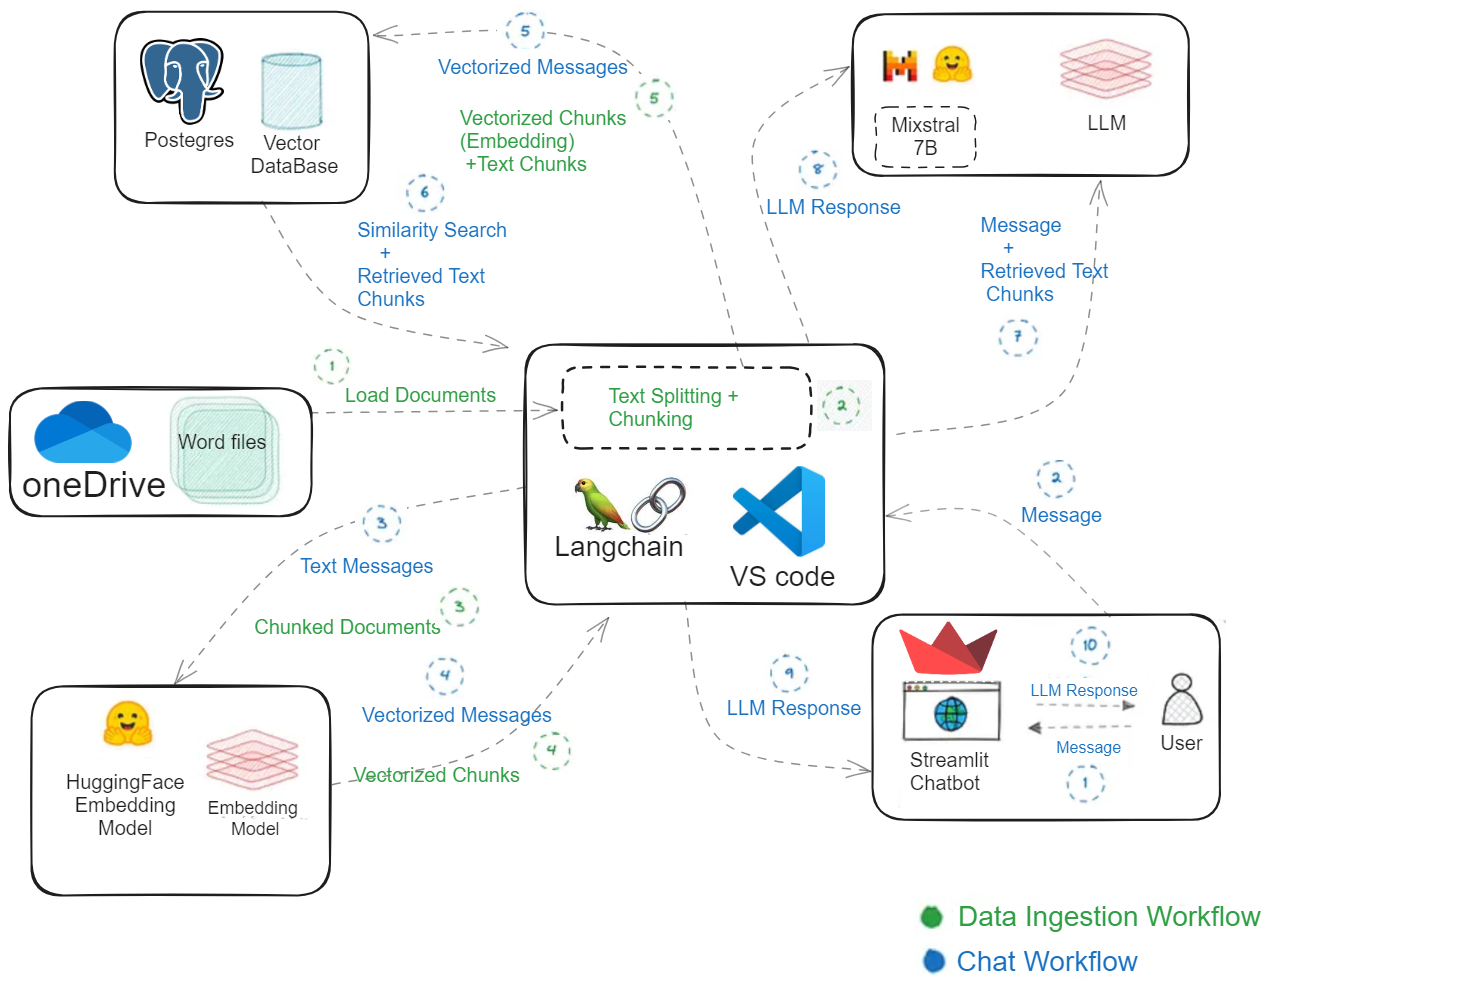
\includegraphics[width=1 \linewidth]{assets/pipeline_rag.png}
    \caption{RAG pipeline}
\end{figure}
The process begins with loading a huge data base or corpus containing relevant information . This information base might contain of content from diverse sources such as books, articles, websites, or any other organized or unstructured data stores.
\vskip 0.5cm
Once the data base is loaded , it s divided into reasonable chunks or sections to encourage effective recuperation . Chunking guarantees that the retrieval process is versatile and doesn t overload the framework with excessive data at once.
\vskip 0.5cm
Each chunk of information is at that point encoded into a numerical representation, ordinarily utilizing methods like word embeddings or more progressed methods such as transformer based models like BERT (Bidirectional Encoder Representations from Transformers) . This vectorization process converts the literary data into high-dimensional vectors that capture semantic and relevant connections between words and expressions.
\vskip 0.5cm
when a query is received , it's also vectorized utilizing the same encoding method as the information base. This grants for effective closeness computation between the query vector and the vectors representing chunks of information inside the information base.
\vskip 0.5cm
Retrieval procedures like approximate nearest neighbor search or other similarity based methods are then employed to recognize the foremost significant chunks of information that match the query vector. chunks of information are recuperated , they are concatenated to make the setting or background data for the discussion . This setting gives the fundamental foundation for creating coherent and pertinent responses.
\vskip 0.5cm
The concatenated context, along with the primary query , serves as input to a large language model such as GPT Generative Pre-trained Transformer or a comparative architecture .
\vskip 0.5cm
large language model creates responses based on the input context and query . By leveraging the pertinent information recovered from the vectorestore. However, the responses are not only fluent and coherent but also grounded in retrieved context.
\vskip 0.5cm
The last response , created by the language model is then displayed to the client or coordinates into the conversational interface.
\vskip 0.5cm
at the end of the process, the generated response is displayed to the client or integrated into the conversational interface. In general, the Rag system consistently integrates the processes of data recovery and generation to create contextually pertinent and coherent responses in conversational applications.
% \begin{itemize}
%     \item \textbf{Message}: The process begins with the user posing a question. This question is the input that needs to be addressed or answered. wich then chunked into vectorized chunks.
%     \item \textbf{Streamlit Chatbot}: This component serves as the essential interface for client interaction with the chatbot. Clients can input their queries here, which the chatbot at that point forms to create and show smart responses . This interaction encourages a consistent communication stream between the client and the chatbot, improving the overall user experience.
%     \item \textbf{Vectorized Chunks}: This term refers to segments of text extracted from a larger corpus that have been converted into embeddings. These embeddings are numerical representations that encapsulate the semantic essence of the text. This transformation enables more efficient and accurate methods for comparing and retrieving information based on content similarity. These are specific segments of text chosen from the corpus by the  Retriever, identified as relevant to the user s message . Their relevance is assessed through the semantic similarity between the embeddings of the user's question and those of the text stored within the vector database. This process ensures that the most pertinent data is retrieved to accurately address the user's needs.
%     \item \textbf{Documents}: These are crucial components within the Rag Retrieval Augmented Generation pipeline. Sourced from various storage solutions like OneDrive or local hardware devices , these documents form the basis for extracting pertinent data . This data is then utilized to make accurate reactions to user inquiries , ensuring that the generated answers are both important and informed.
%     %\item \textbf{Prompt Template}: The relevant chunks and the user question are combined into a prompt template. This template is structured in a way that makes it understandable and usable for a Large Language Model (LLM), preparing it for the query phase.
%     \item \textbf{LLM Query}: The structured prompt is then sent as a query to a Large Language Model. Various LLMs, like those provided by Hugging Face, Cohere, or OpenAI, can be used. This step involves the generative model considering the information from the prompt to generate an accurate and informed response.
%     \item \textbf{LLM Response}: Finally, the Large Language Model generates an answer to the user's question, drawing from the information provided in the prompt and its pre-trained knowledge.
% \end{itemize}


\section{RAG Applications}
Retrieval-augmented generation models have demonstrated versatility across multiple domains. Some of the real-world applications of RAG models are :
\vskip 0.5cm
\begin{itemize}
    \item  \textbf{Advanced question-answering systems}:RAG models can power question-answering systems that retrieve and generate accurate responses, enhancing information accessibility for individuals and organizations. 
    \item \textbf{Content creation and summarization}: RAG models not only streamline content creation by retrieving relevant information from diverse sources, facilitating the development of high-quality articles, reports, and summaries, but they also excel in generating coherent text based on specific prompts or topics.
    \item \textbf{Conversational agents and chatbots}:RAG models enhance conversational agents, allowing them to fetch contextually relevant information from external sources. This capability ensures that customer service chatbots, virtual assistants, as well as other conversational interfaces deliver accurate and informative responses during interactions. Ultimately, it makes these AI systems more effective in assisting users.
    \item \textbf{Information retrieval}:RAG models enhance information retrieval systems by improving the relevance and accuracy of search results.
\end{itemize}
%https://www.google.com/url?sa=t&rct=j&q=&esrc=s&source=web&cd=&cad=rja&uact=8&ved=2ahUKEwidqtXYhoSFAxW6hf0HHRBzDucQFnoECBwQAQ&url=https%3A%2F%2Fhyperight.com%2F7-practical-applications-of-rag-models-and-their-impact-on-society%2F&usg=AOvVaw2zoZR6i6LGVF1jSKhZmGGX&opi=89978449

\section{Conclusion}
%In conclusion, this chapter has offered a comprehensive definition of llm and overview of historical AI story, discussing the common llm types, phases of training and application.Additionally, various LLM tools have been presented, highlighting the usefulness of Langchain over LlamaIndex, as well as existing competing language and embedding models. Finally, this chapter have included the RAG pipeline of our chatbot and its main application.
In conclusion, this chapter has provided a detailed explanation of LLM and a summary of the history of AI. It talks about different types of LLM, how they are trained, and where they are used. It also introduces various tools for LLM and compares Langchain with LlamaIndex, discusses other competing language and embedding models. Finally, this chapter has included the RAG pipeline of our chatbot and its main application.
\vskip 0.5cm
In the next chapter, we will present the chatbot process of the augmented search generation in detail.




\chapter{Chat with PPP data}
%cite{w15} is a problem why?

\section{Introduction}
%This chapter delves into the innovative integration of LLMs (Large Language Models) technology with PPP (Public-Private Partnership) project data. The fusion of AI-driven chat capabilities with PPP data is designed to enhance the feasibility analysis process, providing stakeholders with a more dynamic, interactive, and informed decision-making tool. By leveraging the Retrieval Augmented Generation (RAG) model, this approach aims to significantly improve the precision and relevance of generated responses, tailored to the specific needs and complexities of PPP projects.
This chapter explores the innovative application of Large Language Models (LLMs) combined with Public-Private Partnership (PPP) data in project management. To improve the feasibility analysis process, AI-driven chat capabilities are integrated with PPP data, offering stakeholders a dynamic, interactive, and informed decision-making tool. Additionally, a Retrieval Augmented Generation (RAG) model is employed to enhance the precision and relevance of the responses generated, specifically tailored to meet the unique needs and complexities of PPP projects.
\section{Problem}
%Public-Private Partnership (PPP) projects generate vast amounts of data, from detailed financial reports to comprehensive performance reports. Analyzing this wealth of historical data for insights is a formidable challenge, crucial for refining future PPP ventures. Traditional data analysis methods are often inadequate due to the sheer volume of data, leading to potential oversights and a failure to harness valuable lessons learned.
PPP projects create a lot of information, like financial and performance reports. Studying all this old information to find helpful ideas is a big task, important for improving upcoming partnerships. Traditional data analysis methods may not be enough because of too much data, which can cause important information to be missed or not used effectively. 
\vskip 0.5cm
%Moreover, the relevance of data from past projects diminishes without the ability to adapt insights to the evolving landscapes of regulations, market conditions, and technological advances. As a result, critical decision-making, risk management, and project planning suffer, impacting the efficiency and success of future PPP initiatives.
Furthermore, data from old projects becomes less useful without being able to apply lessons to new rules, market changes, and technology progress. As a result, important choices, making sure things go smoothly, and planning future projects are affected, which makes it harder for future PPP initiatives to be successful.
\vskip 0.5cm
%Addressing this problem requires a novel solution capable of digesting extensive historical data and extracting pertinent insights efficiently. Chatbots, especially those powered by advanced AI algorithms, emerge as a promising solution. They can automate the analysis of large datasets, offer real-time insights, and adapt learnings to the specific context of new PPP projects. By leveraging chatbots, stakeholders can unlock the full potential of their historical data, guiding more informed and effective future project planning and execution. But we must decide what is the best type of chat-bot to use based on our dataset.
To solve this problem, we need a new idea that can analyze a lot of old information and find important information quickly. Chatbots, especially those powered by advanced AI algorithms, are becoming a very good solution. They can automate the analysis of big sets of data, provide immediate insights, and adjust learnings to the specific situation of new PPP projects. By using chatbots, people can make the most of their old data and make better plans for future projects. But we must choose the best type of chat bot to use based on our information.
\section{The Dataset}
Our dataset,a sample was shown at \textbf{Figure \ref{fig:dataset}}, taken from PPP projects, is mostly semi-structured, with Word documents that have text, tables, and images. This type has unique features and information that make it difficult to manage and analyze data efficiently.
%Our dataset, derived from Public-Private Partnership (PPP) projects, is fundamentally semi-structured, containing Word documents that integrate text, tables, and images. This variety poses distinct challenges in data management and analysis, given the unique attributes and insights each data type offers.
\vskip 0.5cm
\begin{figure}[H]
    
    \centering
    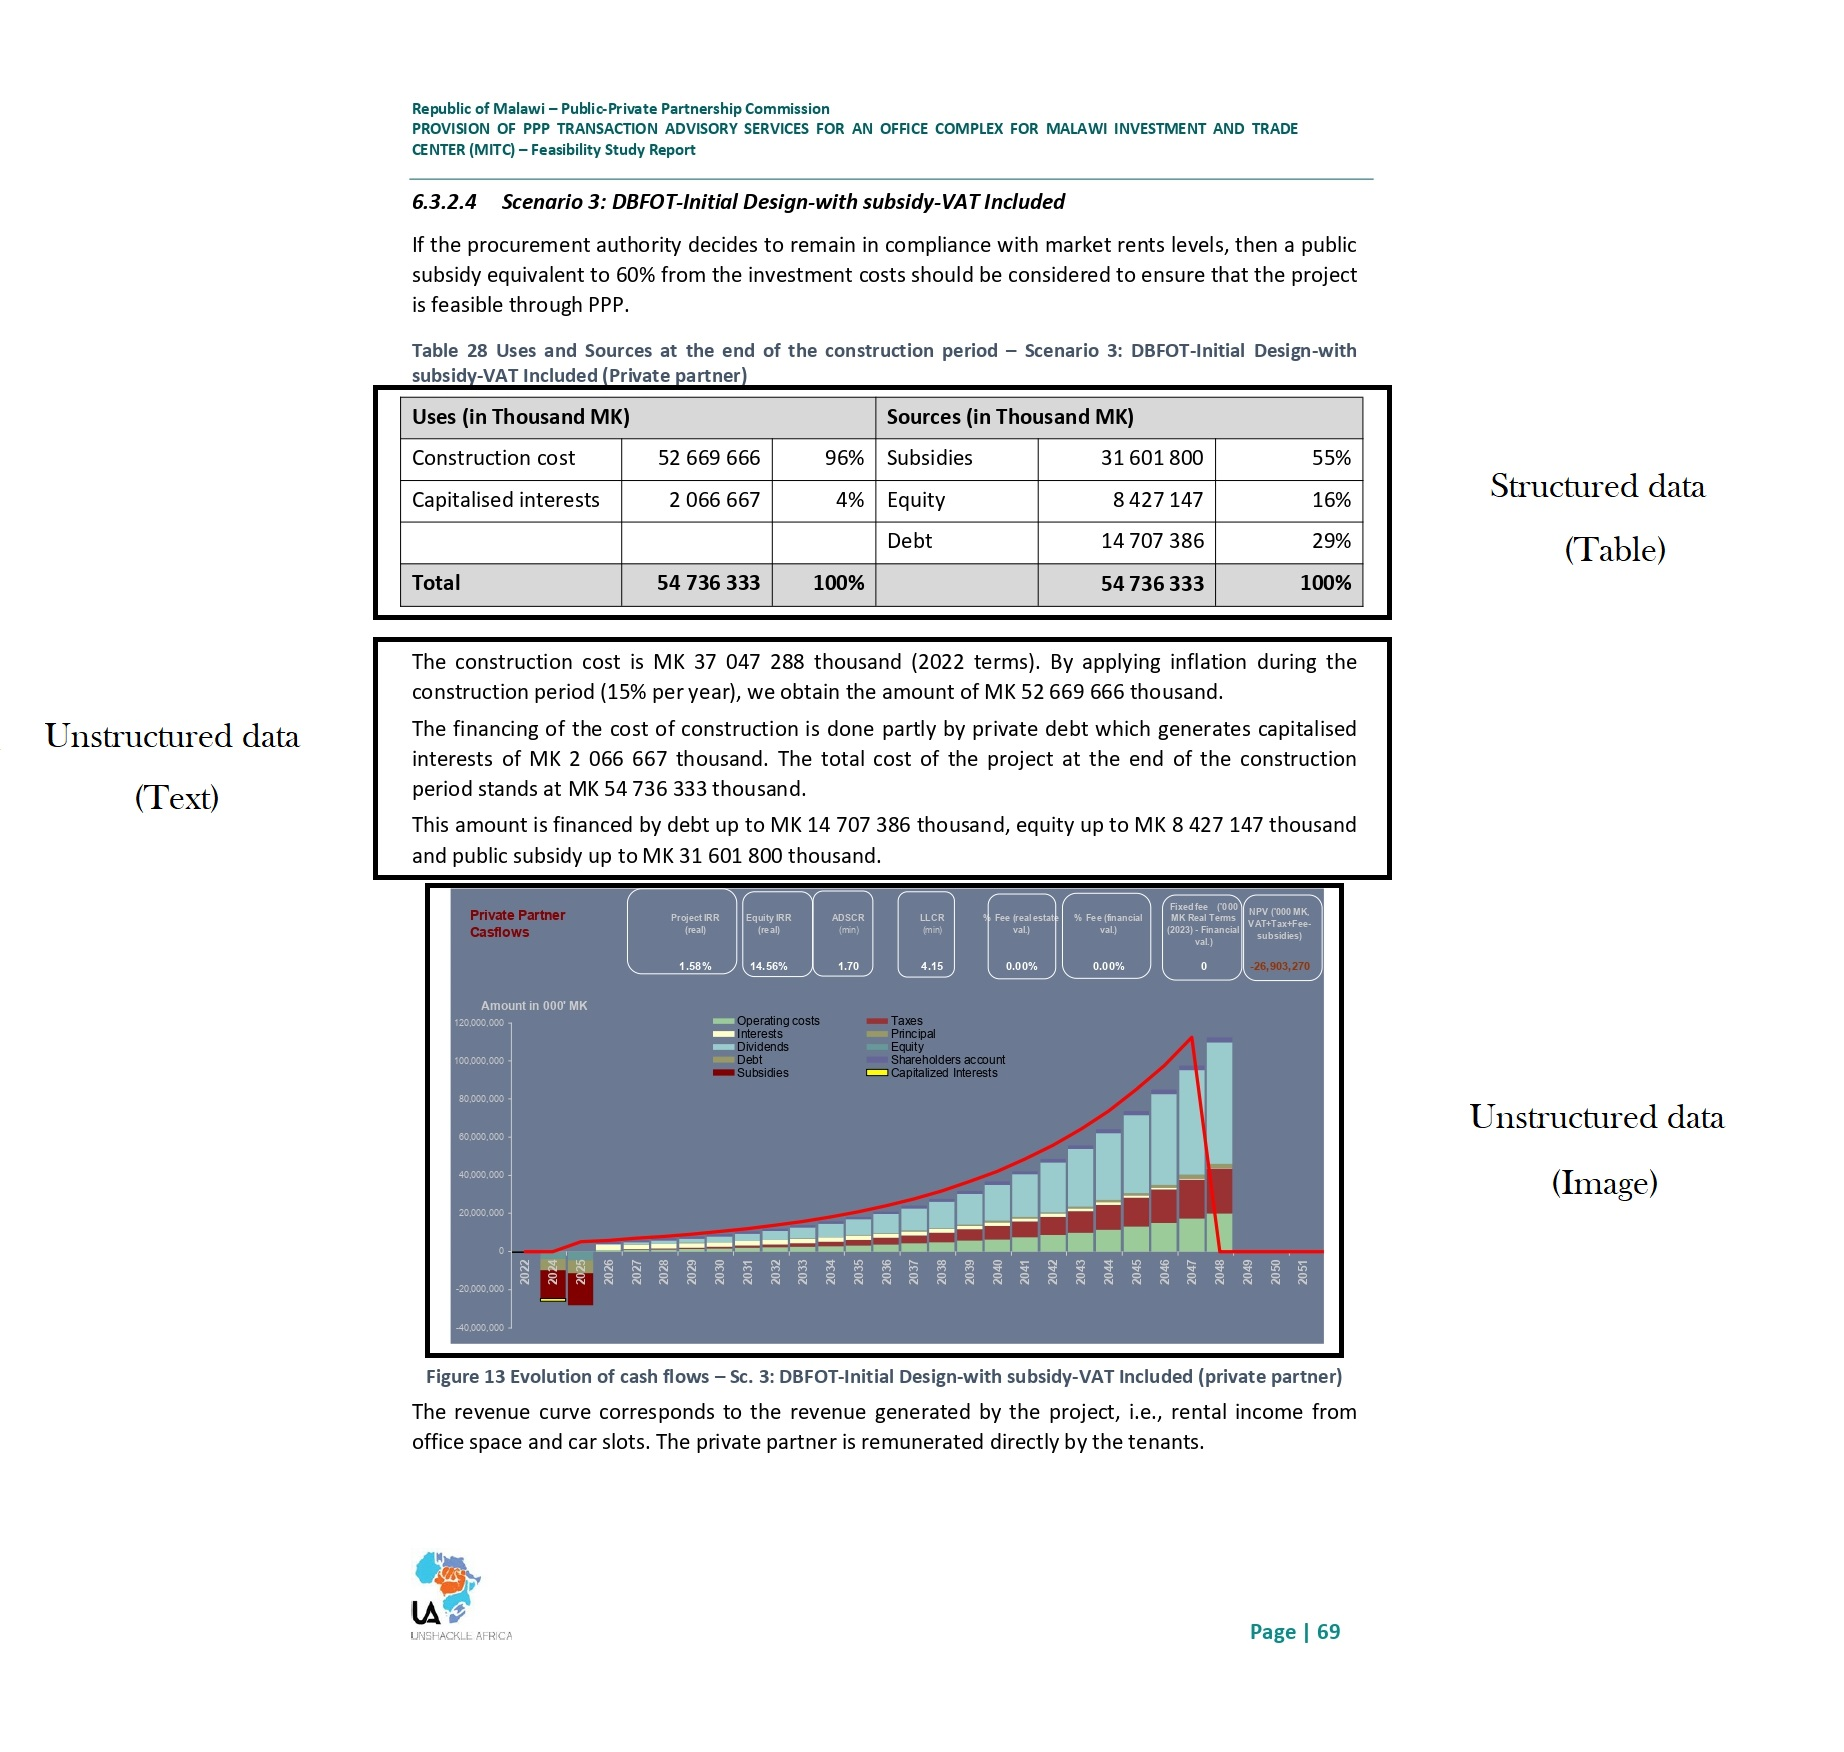
\includegraphics[width=1 \linewidth]{assets/data_ex_page-0001.jpg}
    \caption{Example of a dataset page}
    \label{fig:dataset}
\end{figure}
\vskip 0.5cm
Text: The textual data The textual data includes all the information about projects, contracts, reports on progress, and messages to people involved in the project. The text is full of details but it's hard for computers to understand because it doesn't have a clear structure. Understanding and interpreting detailed documents to find useful information can be difficult because of the complex language and jargon used in PPP projects.
%Text: The textual data includes detailed project descriptions, contracts, progress reports, and stakeholder communications. While rich in narrative detail, the text presents a challenge for automated processing due to its unstructured nature. Extracting specific insights or actionable information from lengthy documents requires sophisticated understanding and interpretation, often complicated by the technical language and specific jargon used in PPP projects.
\vskip 0.5cm
Tables: Embedded within documents, tables give important, organized information about finances, schedules, and performance indicators. The issue comes from the different ways the tables are set up and used in the text. Automated tools need to figure out and take out important information without losing the meaning given by the surrounding text, which can be difficult because of the different layouts and designs used in documents.
%Tables: Embedded within the documents, tables provide crucial, structured data on financials, schedules, and performance indicators. The problem arises in the inconsistent formatting and contextual embedding of these tables. Automated tools must discern and extract relevant data without losing the context provided by accompanying text, a task complicated by the varied layouts and designs employed across documents.
\vskip 0.5cm
Pictures: Pictures, like project drawings, graphs, and photos of the site, give important information about how the project is going and what the results are. Their study is limited because they require special processing methods. Taking information from pictures, especially when it has words or complicated visuals, needs high-tech OCR and image recognition tools, which may have trouble with picture quality, direction, and combining visual data with text and tables.
%Images: Images, including project visualizations, charts, and site photographs, offer valuable insights into project progress and outcomes. However, their analysis is hindered by the need for specialized processing techniques. Extracting data from images, particularly when it involves text or complex visual information, requires advanced OCR and image recognition technologies, which can struggle with image quality, orientation, and the integration of visual data with textual and tabular information.
\vskip 0.5cm
The variety and semi-structered data of our dataset show how complicated it is to analyze data from PPP projects. The difficulties include:
%The diversity and semi-structured nature of our dataset underscore the complexities inherent in PPP project data analysis. The challenges include:
\vskip 0.5cm
Data Integration: Combining information from text, tables, and pictures to better understand project progress and results.%Combining insights from text, tables, and images into a coherent understanding of project statuses and outcomes.
Context Preservation: Keeping the connections between different types of information, like the story behind a table or the details about an image, is very important for getting the analysis right.%Maintaining the context between data types, such as the narrative explanation of a table or the description tied to an image, is crucial for accurate analysis.
Format Variability: There are many different types of documents that need flexible tools to deal with them.
Technical Language: The terminology and common terms in PPP papers need really smart AI tools to understand them correctly.
\vskip 0.5cm
%Addressing these challenges requires a nuanced approach to data processing and analysis, emphasizing the need for advanced tools like chat bots capable of navigating the complexities of semi-structured PPP project data.
Dealing with these challenges requires advanced tools like chat bots that can handle complex PPP project data in a nuanced way. This helps in processing and analyzing data effectively.

\section{Types of Chat-bots}
In the context of managing and analyzing PPP data, it is important to know the different types of chatbots that you can use. These can be put into two groups: rule based chatbots and AI driven chatbots. Each one has its own specific uses and levels of difficulty and flexibility.
%In the context of managing and analyzing Public-Private Partnership (PPP) data, understanding the different types of chatbots available is crucial. These can be broadly categorized into rule-based chatbots and AI-driven chatbots, each serving unique purposes and offering varying levels of complexity and adaptability:
\vskip 0.5cm
\begin{itemize}
\item \textbf{Rule-Based Chatbots:} These chatbots work based on a specific set of rules. They are designed for simple and predictable conversations. Rule-based chatbots excel in scenarios where queries fall within a well-defined range, making them efficient for FAQ-style interactions. However, using to analyze PPP data is difficult because the data is complex and can vary a lot. They are not able to handle unstructured data or give insights beyond their set rules.
%Rule-Based Chatbots: These chatbots operate on a set of predefined rules. They are designed to handle straightforward, structured conversations where responses can be predicted. Rule-based chatbots excel in scenarios where queries fall within a well-defined range, making them efficient for FAQ-style interactions. However, their application in analyzing PPP data is limited due to the complexity and variability of the data involved. They lack the flexibility to process unstructured data or provide insights beyond their programmed rules.
\vskip 0.5cm
\item \textbf{NLP-Driven Chatbots:} AI-driven chatbots, powered by machine learning and natural language processing NLP , can understand and interpret the nuances of human language. Unlike their rule based counterparts, they learn from interactions to improve their understanding over time, making them capable of handling unstructured data. In the world of PPP projects, AI-powered chatbots can look at a lot of insights, find patterns, and get useful information from previous project documents. Their skill in handling and understanding lots of difficult data makes them great at giving personalized advice and predicting future outcomes for projects.
%AI-Driven Chatbots: Powered by machine learning and natural language processing (NLP), AI-driven chatbots can understand and interpret the nuances of human language. Unlike their rule-based counterparts, they learn from interactions to improve their understanding over time, making them capable of handling unstructured data. In the realm of PPP projects, AI-driven chatbots can analyze extensive datasets, identify patterns, and extract actionable insights from past project documentation. Their ability to process and learn from large volumes of complex data makes them particularly suited for offering tailored advice and predictive analytics for future projects.
\vskip 0.5cm
\item \textbf{Hybrid Chatbots:} Using elements from two different methods, hybrid chatbots can answer simple questions using set rules and switch to more advanced answers using artificial intelligence for harder questions. This method ensures that we handle basic questions efficiently and consistently, while still having the ability to dig deeper into data and generate insights for PPP projects.
%Hybrid Chatbots: Combining the best of both worlds, hybrid chatbots utilize rule-based systems for handling routine inquiries and switch to AI-driven responses for more complex questions. This approach ensures efficiency and consistency in dealing with standard queries while retaining the flexibility to engage in more sophisticated data analysis and insight generation related to PPP projects.
\vskip 0.5cm

\item \textbf{Retrieval-Augmented Generation (RAG) Chatbots:} RAG chatbots are a type of AI chatbots that are really good at finding information from a big database before coming up with answers. Chatbots use information from previous projects to give helpful advice and predictions about future projects. Their ability to access historical data archives makes them extremely useful for understanding complicated PPP data environments.
%Retrieval-Augmented Generation (RAG) Chatbots: A subcategory of AI-driven chatbots, RAG chatbots specialize in retrieving information from a vast database before generating responses. By consulting specific data points from past PPP projects, these chatbots can provide highly relevant and context-aware insights, advice, and foresight on potential project outcomes. Their capability to tap directly into historical data archives makes them invaluable for deciphering complex PPP data landscapes.
\end{itemize}
\vskip 0.5cm
In the context of tackling the challenges presented by PPP data analysis, AI-driven and RAG chatbots hold the most promise. Their ability to process and learn from unstructured data, combined with the capability to retrieve and utilize specific information from large datasets, positions them as powerful tools for extracting insights from historical PPP project data. This, in turn, can significantly enhance decision-making and strategic planning for future projects.

\section{Why RAG}
Retrival Augmented Generation RAG mixes the Advanced text-generation skills of GPT and other large language models with information searching features to give correct and contextually relevant information. This new method helps language models better understand and respond to user questions by using the most up-to-date information available. As RAG grows, its many uses are going to change how well AI works and how useful it is.
%Retrieval Augmented Generation (RAG) combines the advanced text-generation capabilities of GPT and other large language models with information retrieval functions to provide precise and contextually relevant information. This innovative approach improves language models' ability to understand and process user queries by integrating the latest and most relevant data. As RAG continues to evolve, its growing applications are set to revolutionize AI efficiency and utility.
\vskip 0.5cm
%In general, General-purpose language models are pre-trained on vast amounts of data from everywhere. But this doesn't mean that it knows the answer to every question. General LLMs fall short in cases like up-to-date or relevant information, domain-specific context, fact-checking, etc. That's why they're called general-purpose and need the assistance of other techniques that are widely implemented to make LLMs more versatile.
%Therefore, we address these shortcomings by integrating information retrieval mechanisms, enabling language models to access external knowledge sources for more accurate and relevant responses, thus mitigate hallucination and strengthen reliability.
In general, General-purpose language models are trained on a lot of data from everywhere. But doesn't mean it knows the answer to every question. Traditional LLMs lack important things like current or important information, specific context, fact checking, etc. That's why they re-called general purpose and need the help of other widely used techniques to make LLMs more versatile.
So, we fix these problems by adding ways for language models to find information, so they can give better and more specific answers. This helps prevent them from making things up and makes them more trustworthy.

\section{Our RAG Components and Pipeline}
%In this section, we will examine the intricate components and sequential processes that constitute our Retrieval-Augmented Generation (RAG) pipeline. We managed to create this pipeline after many iterations of testing and evaluation so we can have the best results. This pipeline stands at the core of our chatbot's ability to navigate through and interact with the multi-faceted data associated with Public-Private Partnership (PPP) projects. It is a harmonious interplay of extraction, indexing, retrieval, fusion, and generation modules, each fine-tuned to handle the semi-structured nature of the PPP data sets, which include text and tables within Word documents, we can see the pipline in figure 4.1.
In this part, we will look at the detailed parts and steps that make up our Retrieval Augmented Generation RAG pipeline. We made this pipeline after lots of testing and evaluation to get the best results. This pipeline is crucial for our chatbot to move through and communicate with the complex data linked to Public Private Partnership PPP projects. It is a smooth combination of different parts that work together to process PPP data sets, which contain text and tables within Word documents. \textbf{Figure \ref{fig:our_rag}} shows the pipeline.
\begin{figure}[H]
    \centering
    \includegraphics[width=1 \linewidth]{assets/our_rag.png}
    \caption{Our RAG pipline}
    \label{fig:our_rag}
\end{figure}

Based on this pipline, in this chapter we will talk about:
\vskip 0.5cm
\begin{itemize}
\item \textbf{Data Extraction and Preparation:} This step involves identifying and extracting out different types of information from Word documents. This includes text and tables. The process makes sure that all important information is gathered and ready for the next steps.%This step involves identifying and extracting varied data types from the Word documents, including text and tables. The process ensures that all relevant information is captured and prepared for the subsequent steps in the pipeline.
\vskip 0.5cm
\item \textbf{Data Embedding}: After extraction, the data goes through a process called embedding. This changes the information into numbers that AI can easily understand and work with. This embedding is very important for capturing the meaning of the data in a way that machines can understand and use it effectively. %After extraction, the data undergoes embedding, where it is transformed into a numerical representation that can be efficiently processed by AI algorithms. This embedding is crucial for capturing the semantic richness of the data in a form that machines can understand and work with.
\vskip 0.5cm
\item \textbf{History-Aware Conversation Management}: At this point, the system uses past interactions to keep track of the conversation flow. This makes sure that each question is based on the history of the conversation, giving a smooth and relevant experience for the user.%At this stage, the system leverages the context of previous interactions to maintain a history-aware conversation flow. This ensures that each query builds on the last, providing continuity and relevance to the user's ongoing experience.
\vskip 0.5cm
\item \textbf{Integrated Retrieval, Indexing, and Re-Ranking}: This system begins by retrieving data from out vector store based on the users question. The retrieval process is integrated with a creative technique known as RAG Fusion. During this phase, the retrieved data is re-ranked by importance, which enhances the quality and relevance of the information used for generating answers. This integrated approach ensures efficient data handling and improved response generation for the user.
\vskip 0.5cm
\item \textbf{Answer Generation}: The last stage of the process where the chatbot puts together the re-ordered information to create complete and relevant answers. The process uses language models and data to give accurate answers to user questions.%The final step of the pipeline where the chatbot synthesizes the re-ranked data to generate comprehensive and contextually relevant responses. The generation process combines the power of language models with the specificity of retrieved data to produce accurate and informative answers to user inquiries.
\end{itemize}
\vskip 0.5cm
%This refined pipeline provides a systematic approach for transforming semi-structured PPP project data into actionable insights through a conversational AI interface. Each step is designed to handle the complexity of the data and the nuances of user interactions, ensuring that the chatbot is not only responsive but also deeply informative.
This advanced pipeline helps to change semi structured PPP project information into useful insights using a conversational AI interface. Each step is made to deal with the difficulty of the data and the details of how users interact, making sure that the chatbot is not just quick to respond but also very informative.
%https://medium.com/@sandyeep70/understanding-rag-evolution-components-implementation-and-applications-ecf72b778d15

%---------------------------------------
\section{Data Extraction and Preparation}
The text extraction stage is important in the RAG pipeline. Here, the AI system works with the Word document to find and separate all the text. This process is intricate and has many steps to make sure the text data is accurate and ready to be used.
%The text extraction stage is a critical part of the RAG pipeline where the AI system interacts with the Word document to identify and isolate the full textual content. This process is intricate and involves several steps to ensure the text data is accurate and ready for interaction.
\vskip 0.5cm
The extraction process is divided into two distinct sub-tasks, one devoted to text extraction and processing  and the other focused on tables extraction and processing This section allows essential control of each type of data, making the extraction process more accurate and efficient. By carefully analyzing textual content and tabular data, the system can gather broader perspectives and enhance its knowledge base, ultimately increasing its ability to provide contextual responses.

\subsection{Text extraction and processing}
The extraction process is divided into two parts, one for extracting and processing text, and the other for tables. This helps make sure the data is extracted accurately and quickly. By looking closely at written words and table data, the system can learn more and improve its knowledge. This helps it give better answers in different situations.
%The initial phase of the RAG pipeline's text interaction involves the comprehensive extraction and meticulous cleaning of textual content from the PPP documents, ensuring that the data fed into the system is of the highest quality and relevance.
\vskip 0.5cm
\begin{itemize}
\item \textbf{Full Text Extraction}: This process begins with a thorough scan of the entire Word document. Sophisticated algorithms are used to go through the document's complicated structure and capture all parts that have text. This means looking closely at all parts of the document, like the main text, titles, footnotes, and extra information on the side. Every paragraph, heading, and written note is carefully taken out, making sure no important information is missed.%This process starts with a deep scan of the entire Word document. Advanced parsing algorithms are deployed to navigate through the complex structure of the document, capturing every element that contains text. This includes diving into the main body, headers, footers, and side notes. Every paragraph, heading, and written note is meticulously extracted, ensuring no potential insight is left behind.
\vskip 0.5cm
This step is crucial because it sets the foundation for the kind of information the chatbot will have available. It is done carefully to capture the detailed story in PPP documents, like project goals, timelines, stakeholder duties, and legal rules.
%This step is crucial as it lays the groundwork for the kind of information the chatbot will have at its disposal. It is performed with precision to capture the nuanced narrative often present in PPP documents, which may include project goals, timelines, stakeholder responsibilities, and legal clauses.
\vskip 0.5cm
\item \textbf{Content Cleaning}: After getting the extracted data, an important cleaning process starts. It involves going through the text to find and delete parts that don't give important information, like the Table of Contents, index, bibliographies, and appendices. Automated scripts are designed to ignore certain parts and focus on the important details of the project.%Following the extraction, a critical cleaning process is initiated. It involves sifting through the extracted text to identify and remove sections that generally do not contribute valuable insights, such as the Table of Contents, index, bibliographies, and appendices. Automated scripts are tailored to recognize and skip over these segments, focusing instead on the substantive content that directly pertains to the project's details and outcomes.
\vskip 0.5cm
The cleaning also includes getting rid of any repeated headers and footers that show up on every page of the document. Moreover, acknowledgment sections and references are not necessary for the chatbot's data analysis and have been left out of the extracted content.
\vskip 0.5cm
\item \textbf{Handling Multilingual Text}: A special problem occurs when the documents are in languages other than English. For example, if the PPP documentation is in French, the system uses Argos Translate, a free, offline translation tool, to change the text into English. "We chose Argos Translate for privacy reasons and to be able to work without needing internet services."%A particular challenge arises when the documents are in languages other than English. For instance, if the PPP documentation is in French, the system employs Argos Translate, an open-source, offline translation tool, to translate the text into English. The choice of Argos Translate is deliberate to ensure data privacy and the ability to operate without reliance on external internet-based services.
\vskip 0.5cm
The choice to use machine translation instead of multilingual embeddings is based on a study by the GDELT Project in their article "Embedding Models: Multilingual Embedding Versus Machine Translation + English Embedding". The study in the article shows that translating non English text into English before embedding works better than using separate embedding models for each language.\textbf{ The figure \ref{fig:comp_multilingual}}, extracted from the article, outlines a comparison between Multilingual Embeddings and Machine Translation then English Embeddings over different dialects , counting Arabic, Chinese, Thai, Russian, German, Spanish, Korean, and Turkish with the same embedding model. As portrayed , the results clearly favor Machine Translation + English Embedding for accomplishing more precise clustering and regrouping of diverse sentences.
%The decision to utilize machine translation over multilingual embeddings is informed by insights from an analysis presented by the GDELT Project in their article "Embedding Models: Multilingual Embedding Versus Machine Translation + English Embedding". The analysis in the article underscores the effectiveness of translating non-English text into English before embedding, as opposed to using separate embedding models for each language.
\begin{figure}[H]
    \centering
    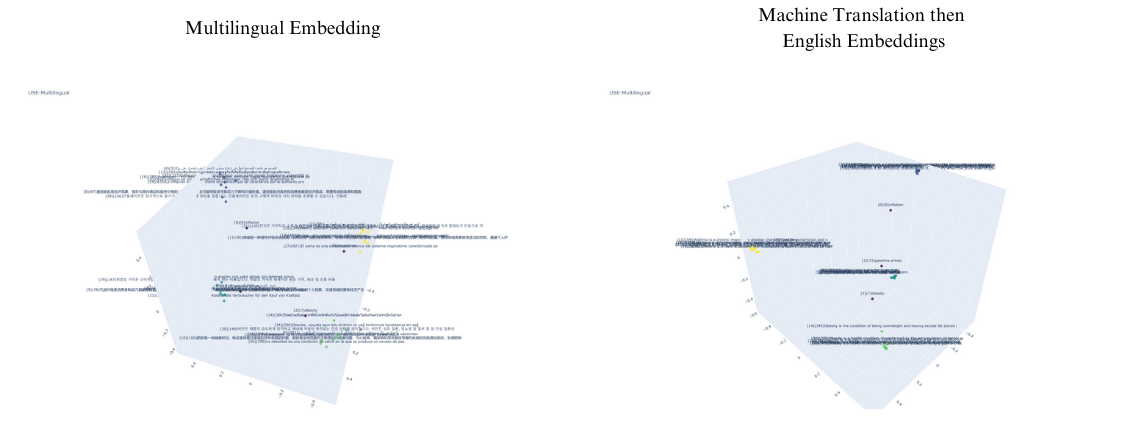
\includegraphics[width=1 \linewidth]{assets/comp_multi.png}
    \caption{comparison between Multilingual Embeddings and Machine Translation then English Embeddings over different dialects}
    \label{fig:comp_multilingual}
\end{figure}
\vskip 0.5cm
By translating all words to English and then using English language embeddings, the system makes sure that the language model can use its training effectively and give the best responses in the RAG pipeline.
%By translating all text into English and then applying English language embeddings, the system ensures that the language model can fully leverage its training and provide the most accurate and informative responses possible within the RAG pipeline.
\end{itemize}
\subsection{Table extraction}
In the RAG pipeline, extracting tables involves carefully finding and getting data from tables, as well as keeping the titles or captions that give information about the tables.
%Table extraction within the RAG pipeline is a meticulous process that involves not only the identification and retrieval of tabular data but also the preservation of its descriptive context, typically provided by accompanying titles or captions.
\vskip 0.5cm
\begin{itemize}
\item \textbf{Identifying and Extracting Tables with Titles}: The first step is to scan the Word document for tables, which are important for analyzing PPP projects. Beside every table, the system also takes out the title or caption that goes with it, often found right above the table in the document. The title is important because it gives a summary or focus of the content in the table, serving as a key to understanding the data. By taking out the table and its title together, the system keeps all the information intact. This helps users to know the meaning and importance of the data.The process begins by scanning the Word document for tables, which are often pivotal in conveying structured, quantitative data essential for PPP project analysis. Alongside each table, the system also extracts the associated title or caption, which is frequently located directly above the table in the document. This title is key to understanding the table's content as it often provides a summary or highlights the focus of the tabular data. By extracting the table and its title in tandem, the system retains the full context, allowing users to understand the purpose and implications of the data within.
\vskip 0.5cm
\item \textbf{Transformation into HTML Format}: After a table and its title are extricated, they experience a change into an HTML (Hypertext Markup Language) format . HTML is chosen since of its various leveled structure, which adjusts well with the inalienable structure of tables. It permits for the representation of complex information in a settled , discernable arrange that's both human readable and machine parseable.
\vskip 0.5cm
This change is guided by standards laid out in research on the representation of tabular data for large language models. For example, the approach recommended within the research paper "Table Meets LLM: Can Large Language Models Understand Structured Table Data? A Benchmark and Empirical Study" \cite{w14} serves as a guide for this process. The paper explains ways to show tables better so that the language model can understand and work with them more easily, \textbf{The Figure \ref{fig:html}} from this paper presents the final findings of different types of transformations and their result across different llm table understanding benchmarks.
%This transformation is guided by principles laid out in research on the representation of tabular data for large language models. For instance, the approach recommended in the research paper "Table Meets LLM: Can Large Language Models Understand Structured Table Data? A Benchmark and Empirical Study" \cite{w14} serves as a reference for this process. The paper details methods for effectively representing tables in a manner that improves the language model's comprehension and interaction with tabular structures.
\begin{figure}[H]
    \centering
    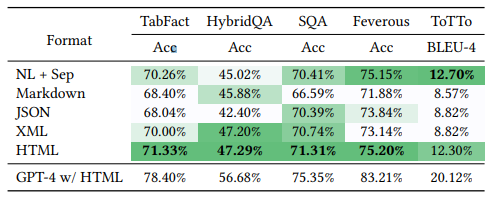
\includegraphics[width=0.9 \linewidth]{assets/html_res.png}
    \caption{Results of different transformations on LLM table understanding benchmarks}
    \label{fig:html}
\end{figure}

\vskip 0.5cm
When we transform tables to HTML format, each part of the table (cell, row, and column) is put inside special HTML tags. This makes a tree like structure that shows the table's layout accurately. The HTML format clearly separates data points, which helps the language model access and understand the table s contents accurately.
%In converting tables to XML, each cell, row, and column is encapsulated within XML tags, creating a tree-like structure that accurately reflects the table's layout. The XML format provides clear demarcations of data points, which is crucial for the language model to navigate and understand the table's contents accurately.
\vskip 0.5cm
\item \textbf{Preparation for LLM Interpretation}: The table is represented in HTML format to help the language model work with tabular data more effectively. This helps the LLM to better use the data from the table during conversations. It gets really good at using and making connections between the tabular data and the text or questions it comes across.%The XML representation of the table ensures that when the language model encounters tabular data, it has a structured and semantically rich format to work with. This enables the LLM to process and integrate the data from the table more effectively into the conversational context. It becomes adept at referencing specific entries and drawing connections between the tabular data and the textual or conversational queries it encounters.
\end{itemize}
\vskip 0.5cm
The RAG pipeline improves the chatbot's ability to use structured data by changing tables and titles into a format that works well with language models. This step makes sure that the chatbot can understand numbers and patterns as well as written words. This helps the chatbot give better and more detailed responses when analyzing PPP projects.
% %By extracting tables along with their titles and converting them into a language model-friendly XML format, the RAG pipeline enhances the chatbot's capability to process and utilize structured data. This step ensures that numerical and structured insights are as accessible and understandable to the chatbot as textual information, leading to more informed and comprehensive responses in the analysis of PPP projects.
% %-----------------------------------------------------

\section{Data Embedding}
Word embeddings are key concept in NLP, a fieldin machine learning. Word embeddings convert text data into numbers that machine learning algorithms can understand. can also help us understand the meaning of words in relation to other words. For example, \textbf{Figure \ref{fig:embed}} shows a example of embeddings in three dimensions. %\cite{w15}.
%Word embeddings are a key concept in natural language processing (NLP), a field within machine learning. Word embeddings transform textual data, which machine learning algorithms can’t understand, into a numerical form they can comprehend. In addition, they can be used to capture the contextual essence of words, their semantic and syntactic similarity, and their relation with other words. For instance, Figure 4.2 illustrates a sample of embeddings in three dimensions\cite{w15}.
\vskip 0.5cm
Before embedding, the document must be divided into smaller sections or chunks, so it can be analyzed and processed more easily. Chunking is play a pivotal role in helping with remembering and creating things quickly. These pieces are then dealt with separately, making it easier to find and create specific information.
%Befor embedding, the document must be broken down into smaller, more manageable segments or "chunks," facilitating focused analysis and processing of the text. the chunking plays a pivotal role in managing the retrieval and generation processes efficiently. These chunks are then processed individually, allowing for more focused retrieval and generation.

\begin{figure}[H]
    \centering
    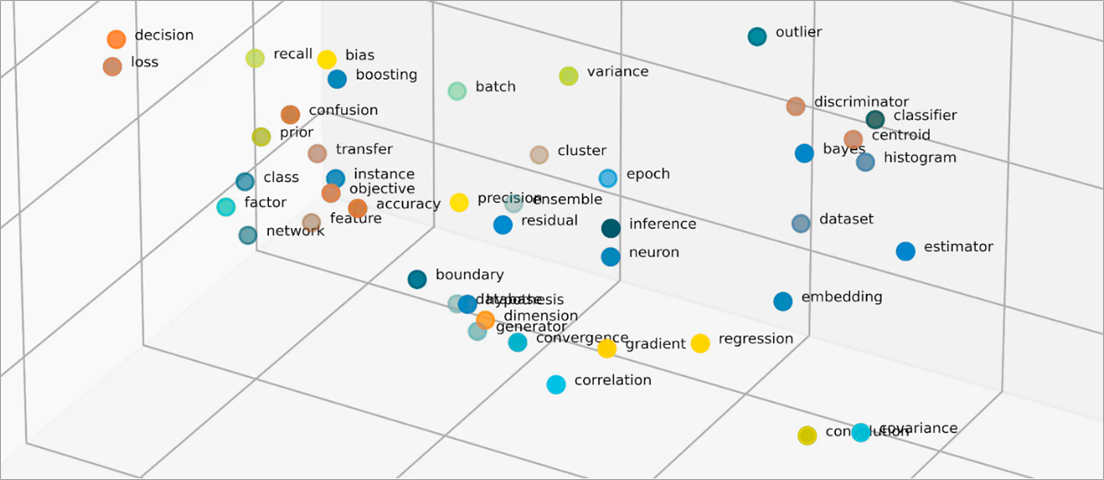
\includegraphics[width=1 \linewidth]{assets/3-d embed.png}
    \caption{Three-dimension embedding sample}
    \label{fig:embed}
\end{figure}
\subsection{Choice of embedding model}
Choosing the right embedding model is very important, especially when working with English documents. The model must be good at understanding the language and specialized terms used in legal and financial documents.
%The choice of the appropriate embedding model is crucial, especially when dealing with documents in the English language. The model must not only accurately capture the nuances of the language but also be adept at interpreting the specialized terminology used in legal and financial documents.
\vskip 0.5cm
The BGE M3 model, mentioned in the article "OpenAI vs. Open Source Multilingual Embedding Models "\cite{w16}, makes a strong argument for why it should be chosen. This model is very good at understanding many different meanings in English because it has been trained on lots of different types of data from lots of different areas. \textbf{The figure \ref{fig:embed_comp}} shows the comparison between different models and their performance on Mean Reciprocal Rank (MRR) which is an evaluation benchmark for embedding models.
\begin{figure}[H]
    \centering
    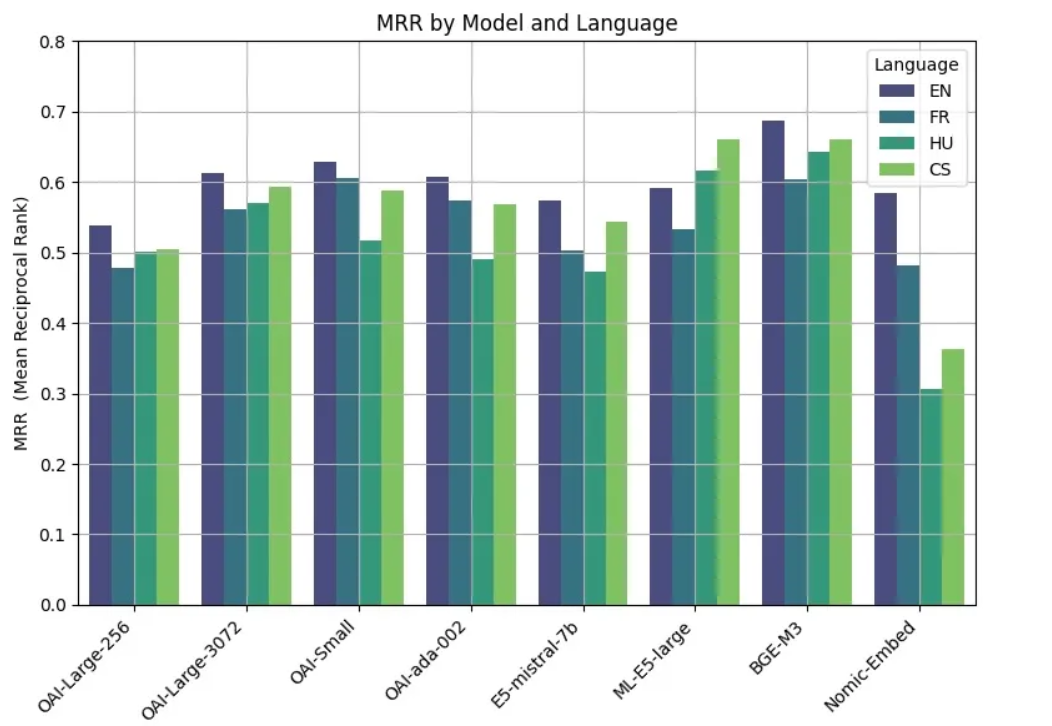
\includegraphics[width=1 \linewidth]{assets/embed_md_comp.png}
    \caption{performance of the latest embedding models on Mean Reciprocal Rank (MRR) benchmark}
    \label{fig:embed_comp}
\end{figure}
%The BGE-M3 model, discussed in the article "OpenAI vs. Open Source Multilingual Embedding Models" \cite{w16}, presents a strong case for its selection. This model is notable for its ability to encapsulate a wide spectrum of nuances in English, given its training on diverse datasets encompassing various domains and contexts.
\vskip 0.5cm
\textbf{Choosing BGE-M3 for English Language Embeddings:} The BGE-M3 model is special because it is part of a group of models that are made to really understand language well, , stands out for several reasons:%The BGE-M3 model, part of the larger family of models that are designed to be both broad and deep in their understanding of language, stands out for several reasons:
\vskip 0.5cm
\begin{enumerate}
    \item \textbf{Model Specifications:} The BGE-M3 model, identified as BAAI/bge-m3, has a dimension of 1024 and can process sequences up to 8192 tokens in length. It is a multilingual model that benefits from a unified fine-tuning approach, incorporating techniques such as dense, sparse, and colbert tuning. These features are derived from its unsupervised learning capabilities, enhancing its versatility and adaptability across various text analyses.
\vskip 0.5cm
\item \textbf{Contextual Understanding:} It has been trained to understand context well, which is important for reading PPP documents that often contains complicated language structures.%It has been trained to comprehend context deeply, which is essential for parsing PPP documents that often contain dense and intricate language structures.
\vskip 0.5cm
\item \textbf{Semantic and Syntactic Awareness:} The BGE-M3 model captures how words are related, which is important when dealing with technical language where accuracy is very important.%The BGE-M3 model captures the semantic relationships between terms, a crucial feature when dealing with technical language where precision is paramount.
\vskip 0.5cm
\item \textbf{Robust Training:} The training process for BGE-M3 has helped the model learn different language patterns, so it can handle new words and ways of speaking easily.%The training regime for BGE-M3 has exposed it to a variety of linguistic patterns, making it robust when dealing with unexpected ways of expression or new terminology.
\vskip 0.5cm
\item \textbf{Efficiency in Processing:} As PPP documents can be very long and complicated, the ability of BGE M3 to process a lot of text quickly is a big benefit, making sure the system stays fast.%As PPP documents can be lengthy and complex, the efficiency of BGE-M3 in handling large volumes of text is a significant advantage, ensuring that the system remains responsive.
\end{enumerate}
\vskip 0.5cm
In summary, the strategic selection of BGE-M3 for English language embeddings helps us analyze PPP project documents better. It makes sure we can use a platform that gives us lots of specific information, context, and accurate insights necessary for informed decision-making.
%In summary, the strategic selection of BGE-M3 for English language embeddings, helps us in providing a nuanced and efficient tool for analyzing PPP project documents. It ensures that we have access to a platform capable of delivering detailed, contextually rich, and accurate insights necessary for informed decision-making.
\subsection{Chunking and embedding for different type of data}
Before embedding, documents are chunked (divided) into smaller segments. This step before the main process is important for controlling the system's workload and helps to find information in a detailed way. Breaking down the text into smaller parts helps the system find and organize information better, making it easier to search for specific content. This approach helps prevent losing important information when dealing with long texts. Each piece of information is carefully looked at.
%Before embedding, documents are chunked into smaller segments. This pre-processing step is instrumental in managing the system's load and allows for a granular approach to information retrieval. By breaking down the text into manageable chunks, each segment can be embedded and indexed individually, which enhances the system's ability to retrieve and generate precise and relevant content. This approach also mitigates the risks of information loss that can occur when handling large blocks of text, ensuring that each piece of information is given due consideration.
\vskip 0.5cm
In our RAG pipeline, Multi Representation Indexing is a very important step where we map different types of data, like text and tables, to their own vector representations. This process makes it easy to find information and ensures you can remember everything.
%In our RAG pipeline, Multi-Representation Indexing is the crucial step where different data types—namely text and tables—are mapped to their respective vector representations. This process allows for a seamless retrieval experience that ensures comprehensive data recall.
\subsection{Tables Chunking and Embedding}
The  multi-representation indexing approach  in our system is designed to handle the complicated table data in PPP documents. Here, the term multi-representation shows that the pipeline can store different types of data, such as vector summaries of tables and the tables themselves.
%The multi-representation indexing approach in our pipeline is designed to effectively handle the complex nature of table data embedded from PPP documents. Here, the term "multi-representation" reflects the pipeline's capacity to index various forms of data, particularly the vector representations of table summaries and the actual tables themselves.
\vskip 0.5cm
\begin{itemize}
    \item \textbf{Process of Indexing Table Embeddings:} When we put the tables into the system, we create vector summaries of the important information in the tables. These summaries are stored in a database called PgVector which can handle vector data. This process involves making a map between a high-dimensional vector space and the original table. Each vector is a point in this space, representing the meaning and information in a table summary. By indexing these vectors, we make it easier to find things quickly when looking for specific information through semantic queries.%Upon embedding the tables, the resulting vector representations — summaries that capture the essential information within the tables — are indexed in a database designed to handle vector data, such as PgVector. This indexing process involves creating a map between the high-dimensional vector space and the original tabular data. Each vector is a point in this space, representing a table summary's semantic and informational content. By indexing these vectors, we facilitate a highly efficient retrieval process, where searching for information through semantic queries becomes possible.
    \item here we choose the llmm (comp table)
    \item \textbf{Retrieval of Full Table Data:} The strength of multi-representation indexing is that it able to link these vectors back to all the data in the table. When a user needs specific information, the system can find the right data and get the complete table. This means that users will get a short answer to their questions and also be able to look at all the detailed information in the table to get a better understanding.%The strength of multi-representation indexing lies in its ability to associate these vectors back to the full table data. When a user's query necessitates specific data retrieval, the system can quickly locate the relevant vector in the indexed space and then pull the complete table from the repository. This ensures that users not only receive a summary response to their queries but can also access the detailed data within the table for comprehensive insights.
\end{itemize}

\subsection{Text Chunking and Embedding}
The sophisticated architecture of our RAG pipeline can handle different types of text data from PPP documents using a method called multi-representation indexing. This means the pipeline can organize various kinds of data, especially focusing on the vector representations of small text pieces and the longer text segments they come from(parent chunck).
%The sophisticated architecture of our RAG pipeline accommodates the varied and layered texture of textual data extracted from PPP documents through a method known as "multi-representation indexing." This term encapsulates the pipeline's ability to meticulously index different forms of data, specifically focusing on the vector representations of small textual chunks and the full-bodied text segments from which they are derived.
\vskip 0.5cm
\begin{itemize}
    \item \textbf{Chunking for Text Embedding:} For this process, we are using Recursive text splitting which involves breaking down a big piece of text into smaller chunks. This is really helpful when working with long documents, because it helps the system to manage and process data while still keeping important information in context.%For this processes we are usign Recursive text splitting which is an iterative process where a larger body of text is progressively broken down into smaller segments or chunks. This is particularly useful when dealing with extensive documents, as it allows the system to manage and process data in a way that balances context retention with manageable analysis sizes.
    \vskip 0.5cm
    The process starts by breaking the document into big chunks, each containing up to 3000 tokens. This initial size of each chunk is set in order to make sure that each part has enough information to accurately show the details of the text.
    %The process begins with the initial splitting of the document into large chunks, each up to 3000 tokens in size. This initial chunk size is chosen to ensure that each segment maintains enough contextual information, which is essential for the embeddings to accurately represent the nuances of the text.
    \vskip 0.5cm
    After this first pass, these large chunks may still be too broad for the fine-grained analysis and retrieval purposes of our system. Therefore, the large chunks undergo a second round of recursive text splitting, where they are further divided into smaller chunks, each consisting of approximately 200 tokens. This size is optimized for the embedding process, where each small chunk is then transformed into a vector representation that captures the semantic richness of the text within that segment.
    \item \textbf{Multi-Representation Indexing:} In our pipeline, both levels of chunked data—large (3000-token) chunks and small (200-token) chunks—are important. The small chunks are embedded and the vectors produced from these embeddings are indexed. However, when it comes to retrieval, the system uses multi-representation indexing to ensure that it can return information from the larger chunks.
    \vskip 0.5cm
    The selection of recursive text splitting and multi representation indexing offers a highly productive approach to handling broad PPP documents. By breaking content into both large and small chunks and embedding these for point by point indexing , the framework adeptly balances comprehensive information analysis with the require for holding relevant information. This technique guarantees that the retrieval process is robust and exact.
\end{itemize}
%definition for the vectorstore its utility and how it helps us for the development of our ai assistance
%how we chose our db 
%what is the differnce between relationnal db and vectorstore.
%etc




\section{History-Aware Conversation with Document}
Within the domain of interactive AI frameworks , the capacity to review and construct upon past saved interactions is fundamental for keeping up a coherent and significant discourse . Typically where History Aware Conversation Management comes into play inside our Rag pipeline, especially within the context of engaging with PPP reports.
\vskip 0.5cm
\begin{enumerate}
    \item \textbf{Selective Document Interaction:} Inside our Rag pipeline, the selection of a particular document to interact with is essential. It engages users to lock in specifically with a specific PPP feasibility report from an established store associated to Jade's OneDrive collection and also save their chat history to our database. The user can choose and search for a report, then they can start a unique conversational thread with that document. This interaction isn't generic but profoundly personalized, permitting the user to inquiry and speak with the content of the chosen report as in case it were a knowledgeable partner. 
    \vskip 0.5cm
    \item \textbf{Question Translation and Reformulation for Context Awareness:} After selecting the document, then the users can pose questions in various languages, the system adeptly translates these into English, using advanced models to ensure nuanced accuracy. This translation is then fused with the document's chat history, providing the large language model (LLM) with a rich contextual backdrop. The LLM may reformulate the inquiry for enhanced context specificity, drawing from previous dialogues and document details to craft questions that elicit more precise information. This consistent use of English across the board maintains the system's processing uniformity, ensuring each user receives context-aware, insightful responses from the conversational AI.
\end{enumerate}

\section{Integrated Retrieval and Re-Ranking}
Within the Rag pipeline, the integrated retrieval and re ranking process plays a essential part in improving the system s response quality. This stage takes after the extraction and embedding stages where both tables and content chunks are indexed and made searchable.
\subsection{Similarity Search on Indexed Documents}
The Similarity Search stage could be a pivotal component of the Rag pipeline, where the system s capacity to accurately and productively coordinate user questions to the most significant information comes into play.
\vskip 0.5cm
\begin{enumerate}
    \item \textbf{Mechanism of Similarity Search:} Upon accepting a query , the system takes the user s input into a query vector utilizing the same embedding model applied to the text and table information during the indexing stage . This vector represents the semantic signature of the query.
    \vskip 0.5cm
    \item \textbf{Finding the Best Match:} The multi representation indexed archives make a searchable space, our vector store (PgVector). Comprising of vectors for each chunk of content and table information. Each vector acts as a arrange in this high dimensional space, encoding the semantic essence of the corresponding text or table.
    \vskip 0.5cm
    The system conducts a search inside this vector space to distinguish the vectors that are closest to the query vector those with the highest degree of semantic similarity . This similitude is regularly computed utilizing metrics such as cosine similarity , which measures the cosine of the angle between two vectors, showing how closely aligned the implications of the query and the archive chunks are. For example, \textbf{Figure \ref{fig:vec_search}} shows a vector representation of kitten query and how it's close to other animals representation especially to cat and dog.
    \vskip 0.5cm
    \begin{figure}[H]
        \centering
        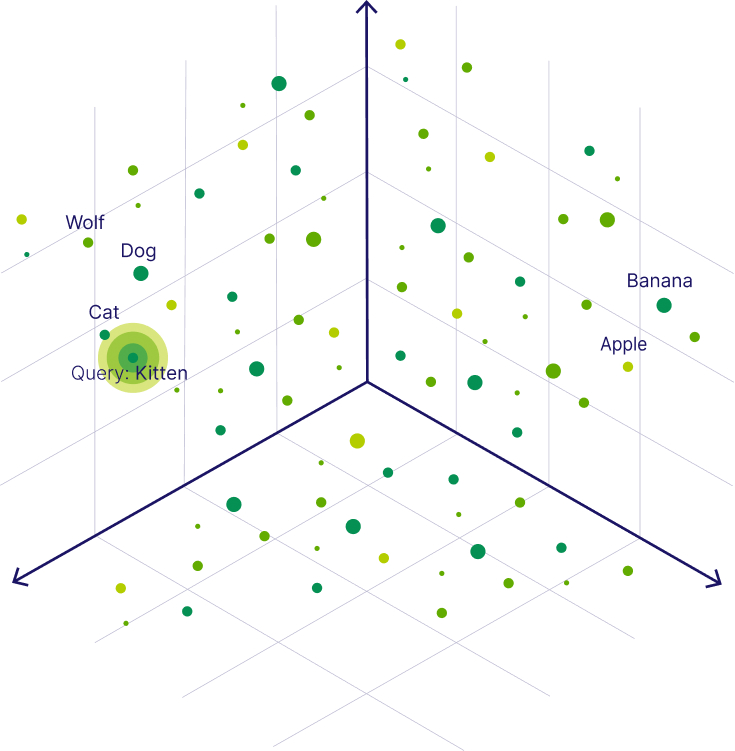
\includegraphics[width=0.8 \linewidth]{assets/vec_search.jpg}
        \caption{Vector representation of kitten query and how it's close to other animals representation in a 3 dimensional space}
        \label{fig:vec_search}
    \end{figure}
    \vskip 0.5cm
    The closest vectors are at that point mapped back to their original content chunks or table information . This retrieval is the primary step in giving a response to the user s query , sourcing the foremost semantically aligned pieces of data from the complete corpus of indexed documents .
\end{enumerate}
The Similarity Search on Indexed Reports may be a confirmation to the power of vector space modeling in understanding and retrieving data. It empowers the system to filter through endless amounts of information with precision and return the foremost pertinent data, hence streamlining the user's experience in exploring complex PPP reports.
\subsection{RAG Fusion for Contextual Alignment}
RAG Fusion is an advanced technique in the RAG pipeline that harnesses the strengths of ensemble methods and reciprocal rank fusion for superior data retrieval.
\vskip 0.5cm
At it's core RAG Fusion uses Reciprocal Rank Fusion (RRF) which is an integral component within the context of Rag fusion that essentially contributes to the efficiency and accuracy of the retrieval process within the pipeline. Its execution inside the Rag system offers a method for combining the strengths of distinctive retrieval models to ensure the foremost important data is surfaced in response to a user's inquiry.
\begin{itemize}
    \item \textbf{Fundamentals of Reciprocal Rank Fusion (RRF):} RRF is based on the principle that the significance of a document can be inversely relative to its positioning over diverse retrieval models. The method was detailed in a research paper by Cormack, Clarke, and Buettcher,titled "Reciprocal Rank Fusion Outperforms Condorcet and Individual Rank Learning Methods"\cite{w17}. It s an successful data fusion strategy that totals different positioned lists into a single, more exact ranking.
    \vskip 0.5cm
    \item \textbf{How RRF Works:} In RRF, each document's rank from the individual result sets is converted into a score using the reciprocal of its rank. This means that if a document is ranked first in any retrieval model's list, it's assigned a score of 1; if it's ranked second, it gets a score of 1/2, and so on. These scores are then summed across all retrieval models for each document. The documents are then re-ranked based on these composite scores, with higher scores indicating higher relevance. This is the RRF equation
    \vskip 0.5cm
    \[
\text{RRFscore}(d \in D) = \sum \left[ \frac{1}{k + r(d)} \right]
\]

\text{where:}
\begin{itemize}
  \item \( d \) represents a document within the set \( D \) of documents.
  \item \( k \) is a constant that helps to balance between high and low ranking documents.
  \item \( r(d) \) is the rank or position of the document \( d \).
\end{itemize}
\item \textbf{Contribution to our RAG Pipeline:} The application of RRF in the RAG pipeline enhances the retrieval process by allowing the system to effectively combine and leverage the insights from our two different retrievals, the text retrieval and table retrieval . This is particularly useful in the RAG framework, where diverse data formats and complex query contexts can lead to varying retrieval performances across different models and with RRF we can have a unified set of score for each chunk returned whether it is a text chunk or a table.
\end{itemize}
\vskip 0.5cm
The RRF method enhances the RAG fusion process by adeptly amalgamating the strengths of varied retrievals, ensuring the system’s effectiveness over diverse datasets. Its application is pivotal in re-ranking the information chunks retrieved, which is essential for furnishing the most contextually relevant and reliable answers to complex inquiries. By reordering these data chunks, RRF helps to align the output more closely with the user's original intent.
\vskip 0.5cm
The effectiveness of RRF in reordering content for LLMs can be further understood through the lens of the research paper "Lost in the Middle: How Language Models Use Long Contexts"\cite{w18}. This study underscores the challenges and solutions in how LLMs handle extended contexts. LLMs are often designed to prioritize information at the top and the end of a user query as being more relevant, which might not always align with the user's needs. We can mitigate this by re-ranking the data chunks, placing those with the highest relevance at the start and end of our query. This tailored reordering can lead to more coherent and contextually rich responses from the LLM. \textbf{Figure \ref{fig:lost_in}} from this study shows how Changing the location of relevant information within the language model’s input context gives different results.
\begin{figure}[H]
    \centering
    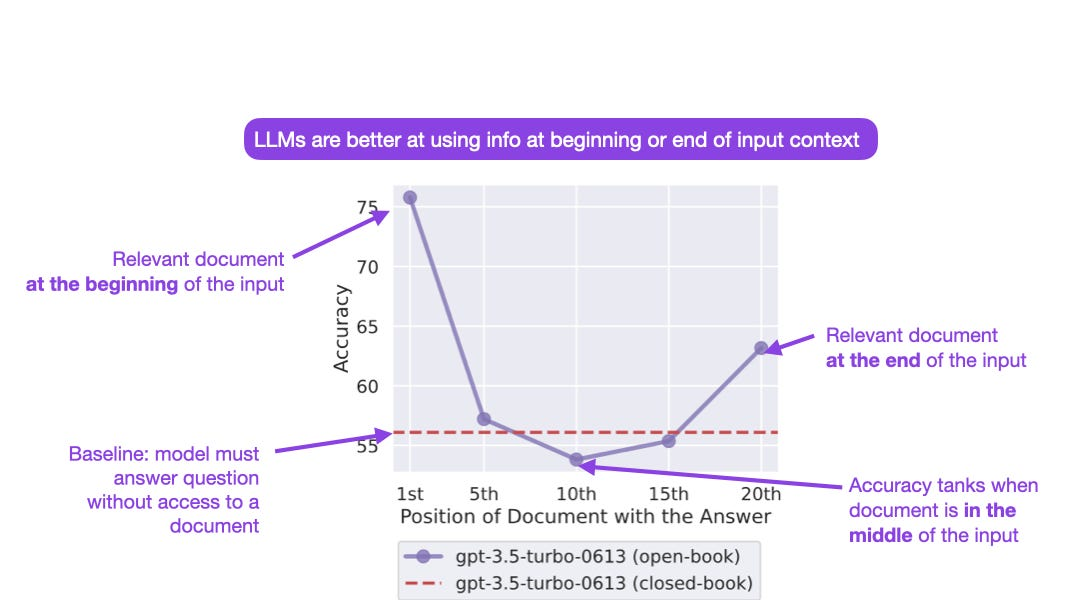
\includegraphics[width=1 \linewidth]{assets/lost_in.jpg}
    \caption{Result of changing the position of the passage that answers an input question}
    \label{fig:lost_in}
\end{figure}
\vskip 0.5cm
In essence, RRF acts as a strategic intermediary in the RAG fusion process, optimizing the arrangement of data chunks fed into the LLM. This optimization facilitates the generation of better-informed answers, effectively harnessing the long-context capabilities of LLMs to provide users with precise and contextually nuanced responses.
\section{Answer Generation}
\section{RAG system Evaluation}
%Explanation of evaluation metrics and methodologies for assessing the performance of RAG systems.
%Presentation of experimental results and analysis of system performance.

\section{conclusion}






\include{./chapters/Chapitre5}
\chapter*{Conclusion Générale}
\markboth{Conclusion Générale}{}
\addcontentsline{toc}{chapter}{Conclusion Générale}

Nous espérons que ce document vous a aidé à rédiger votre rapport convenablement.

Ce document vise à aider les étudiants à rédiger des rapports en Latex.



%
%\bibliographystyle{alpha}
%\bibliography{Biblio}
%\addcontentsline{toc}{chapter}{Bibliographie}% ajouter son entr?e dans la table
\clearpage
\addcontentsline{toc}{chapter}{Notegraphy}
\bibliography{biblio}
\bibliographystyle{ieeetr}
\pagestyle{empty}

\chapter*{Annexe 1}

\addcontentsline{toc}{chapter}{Annexe 1, Les candidats classés par ordre alphabétique}









% Fin du document
\end{document}